% Documentclass options:
%    10pt, 11pt, 12pt  -- set type size
%    draft             -- single space, mark overfull hboxes on paper
%    final             -- double space, don't mark overfull hboxes on paper
%    oneside           -- format for one-sided printing
%    twoside           -- format for two-sided printing
% Defaults are 11pt,final,oneside.  Keep these, please.
\documentclass[11pt]{ucscthesisbs}
\bibliographystyle{apalike2}
\usepackage{natbib}
\usepackage{graphicx,epsf}% Include figure files
\usepackage{spverbatim}


% The following declaration is for citations and bibliographies consistent with
% Astrophysical Journal specifications.  It may be left out or replaced with
% another bibliography/citation style.  See also the "\bibliographystyle"
% command later in this file.
%\usepackage{apj}

\usepackage{xcolor}
\usepackage{pagecolor}
\usepackage{lipsum}  
\usepackage{subfig}
\usepackage{amsmath}
\usepackage[font=small,labelfont=bf]{caption}

% \pagecolor{darkgray}
% \color{white}

\pagecolor{white}
\color{black}


\begin{document}

% Declarations for Front Matter

\title{Thermal Evolution of Uranus and Neptune with Condensation-inhibited Convection}
\author{Robert Schroder}
\degreeyear{2020}
\degreemonth{December}
\degree{BACHELOR OF SCIENCE}
\field{ASTROPHYSICS}%

% Declare up to five committee members.  The text will be reproduced directly
% on the signature page.  Though the chair is a committee member, leave
% him/her out of the \committeemember declarations.  Make sure \numberofmembers
% agrees with the number of committee members declared INCLUDING the chair.
% If it is wrong, you will get extra or missing lines on the signature page.
%
\chair{Bruce Schumm}
\thesisadvisor{Christopher Mankovich}
\technicaladvisor{Jonathan Fortney}
\numberofmembers{2}




\campus{Santa Cruz}

\maketitle
\copyrightpage

\begin{frontmatter}

\begin{abstract}
This will be the last section written, once we have finished our results and conclusion.
\end{abstract}

\tableofcontents
%
% The most recent (10/95) guidelines make absolutely no mention of the list
% of figures and list of tables.  Are they necessary?  If not, comment the
% next two lines out.
%
\listoffigures
\listoftables

\begin{dedication}
\null\vfil
{\large
\begin{center}
To Who,\\\vspace{12pt}
M  ention to who, if anyone, here
\end{center}}
\vfil\null
\end{dedication}

\begin{acknowledgements}
I'd like to thank....
\end{acknowledgements}


\end{frontmatter}

%\part{First Part}

\chapter{Introduction}

During the 1950's, Frank Low observed that Jupiter was radiating away more energy than it received from the Sun \citep{hubbard_1968},\citep{low_1966}. To explain this, physicists set out to develop a theory of interior structure for solar system gas and ice giants \citep{hubbard_1977}, \citep{hubbard_1977_2}, \citep{podolak_1991}. At the present time, most of the giant planets in our solar system: Saturn, Jupiter, and Neptune, all have effective temperatures greater than their equilibrium temperature. Uranus is the exception. Observations of Uranus show a planet that appears to be in thermal equilibrium with its parent star, a planet with no intrinsic temperature, cooler than its more distant neighbor, Neptune, a planet with similar mass and composition. Thermal evolution models for Uranus have not matched observation, instead predicting a warmer effective temperature at $4.6$ Gyr, the current age of the solar system \citep{fortney_2011}, \citep{podolak_1991}, \citep{hubbard_1995}, \citep{scheibe_2019}.

There have been various attempts to explain Uranus' cool temperature. Early investigations posited that a stratified interior, stable against convection, would allow heat to be trapped deep within the the interior \citep{podolak_1991}. Later work built on this idea, investigating the formation of stable condensation zones \citep{friedson_2017}, \citep{leconte_2017}, and \citep{guillot_1995}, and thermal boundary layers \citep{nettelmann_2016}, that could inhibit convection. It was speculated that the presence of these thermal boundary layers, or condensation zones, could trap heat deep within the interior, allowing the envelope above to cool more rapidly, thereby lowering the planet's effective temperature.

\section{Condensation in Hydrogen Dominated Atmospheres}
On Earth, moist air is lighter than dry air. For example, water vapor, the primary condensate in Earth's atmosphere is lighter (not by much) than the background air which is composed primarily of $N_{2}$. Thus, when $H_{2}O$ condenses out of the atmosphere, there is small vertical gradient in mean molecular weight. This small gradient does not impose a significant barrier to convection. By contrast, in hydrogen dominated atmospheres such as Neptune and Uarnus, the background gas is much lighter than the condensates. In this hydrogen-rich environment, when $H_{2}O$ condenses out of the atmosphere, a stong vertical gradient in mean molecular weaight can be established, resulting in a negative bouyancy for the convecting parcel of gas. This can create a situation where the zone in which water condenses is stable against convection \citep{guillot_1995}, \citep{friedson_2017}, \citep{leconte_2017}. 

In this paper, we investigate where and when, assuming a variety deep water concentrations, whether such stable water condensation zones could form within in the outer envelope of the solar system ice giants, and present their potential impact on the thermal evolution of the these planets. We give a brief description of interiror structure models and how our model differs in Chapter 2. We present our results in Chapter 3, describing where and when stable water condensation zones form, and their impact on thermal evolution. In Chapter 4, we discuss our conclusions and offer suggestions for further work.


\chapter{Model}

\section{Three-layer Model with Dry Adiabat}
\label{Three-layer Model with Dry Adiabat}
We begin our description of the physics of our interior structure model starting with the conservation of mass:

\begin{equation}
  \frac{dm}{dr} =4 \pi r^{2}\rho  
\end{equation}
where $dm$ is the mass contained within a sphere of radius $r$, and $\rho(r)$ is the density at radius $r$. Hydrostatic equilibrium is also assumed and described by:

\begin{equation}
  \frac{dP}{dr} = -\frac{Gm\rho}{r^{2}}  
\end{equation}
where $P$ is the pressure and $G$ is the gravitational constant. 

We employ a three-layer interior structure, seen schematically in Figure 2.1. At the center of the planet is a core made of rock and ice. Moving outward, the inner envelope is $H_{2}O$ dominated, with uniform concentrations of $H$, $He$, and $H_{\rm{2}}O$. The outer envelope, below 1 bars, contains trace amounts of $H_{\rm{2}}O$, but is mostly comprised of $H$ and $He$. To accomodate the incredibly high temperatures and pressures experienced deep in the interiror of giant planets, We use the MAZEVET EOS as our $H$-$He$ equation of state \citep{mazevet_2019}. For metals, we use MH13SCVH EOS \citep{miguel_2018}. [How much more should I go into this?]

\begin{figure}[ht!]
 \centerline{
  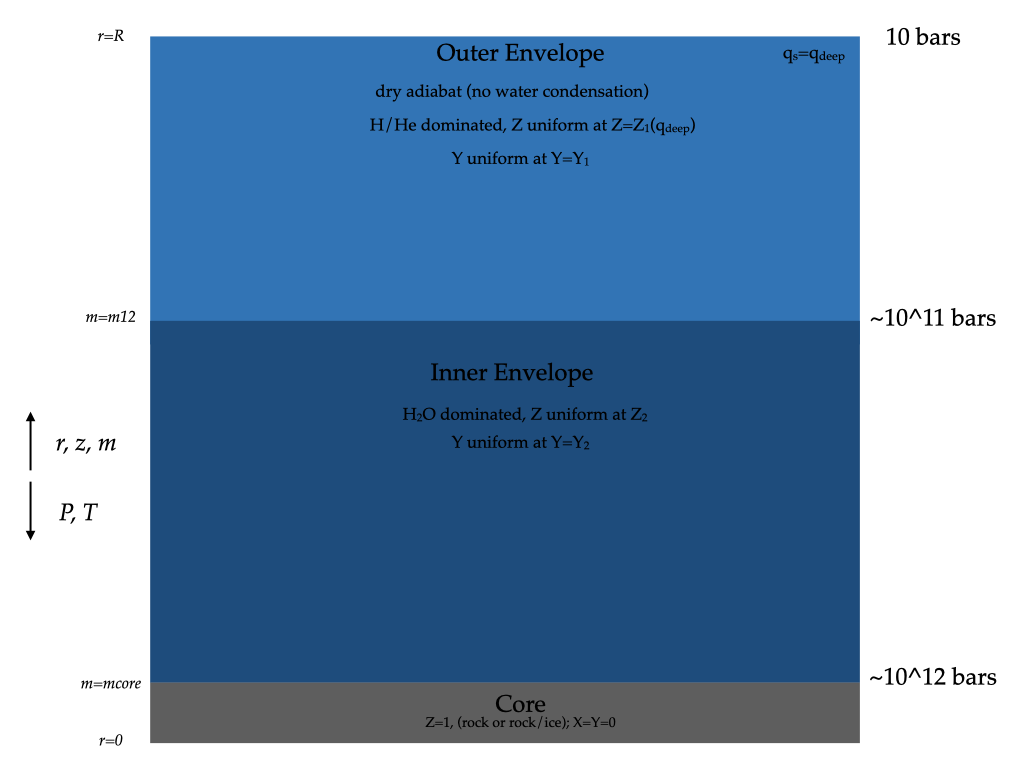
\includegraphics[width=6.0in]{figures/structure_schematic_images/structure_schematic_images.001.png}
 }
\caption[A Standard Interior Structure Model]
{The structure for a fully convective, dry adiabatic interior. In this model, the inner and outer envelopes are assumed to be well mixed, fully convective, and following a dry adiabat. The core is composed of rock and ice. The inner envelope is water dominated, with with uniform concentrations of hydrogen, helium, and water; whereas, the outer envelope is hydrogen and helium dominated, with trace amounts of water. The 'atmosphere' exists above 10 bars.}
\label{fig:standard_dry_interior}
\end{figure}

Historically, interior structure models have assumed that the interiors are composed of compressible gasses that are statically unstable and fully convective. In a dry-convective model such as this, a parcel of gas rises as its temperature increases while its pressure remains constant. This process happens without the addition or loss of heat from the parcel, a process referred to as adiabatic. Furthermore, while there may be a critical concentration for a condensible species, this dry model does not allow for condensation. The temperature-pressure profile follows a dry adiabat gradient \citep{kippenhahn_2012}, given by:

\begin{equation}
  \nabla_{\rm ad} = \left( \frac{\partial \ln T}{\partial \ln P} \right)_{\rm s}
\end{equation}

Finally, beyond the outer envelope is the atmosphere. When modeling the thermal evolution of gas and ice giants, it has long been recognized that model atmospheres constitute an outer boundary condition for interior structure models, providing key inputs that impact cooling times for interior structure models. Our work considered both \citep{graboske_1975} and \citep{fortney_2011} model atmospheres. In this paper, our results will utilize the Fortney 2011 model atmospheres. 

\section{Inclusion of Moist Adiabat Within Outer Envelope}
Our interior structure model modifies the structure described in Section \ref{Three-layer Model with Dry Adiabat} by adding a moist adiabatic layer to the outer envelope, which under favorable conditions, allows for the condensation of $H_{2}O$. We define the moist adiabat as follows \citep{robinson_2016}:

\begin{figure}[ht!]
 \centerline{
  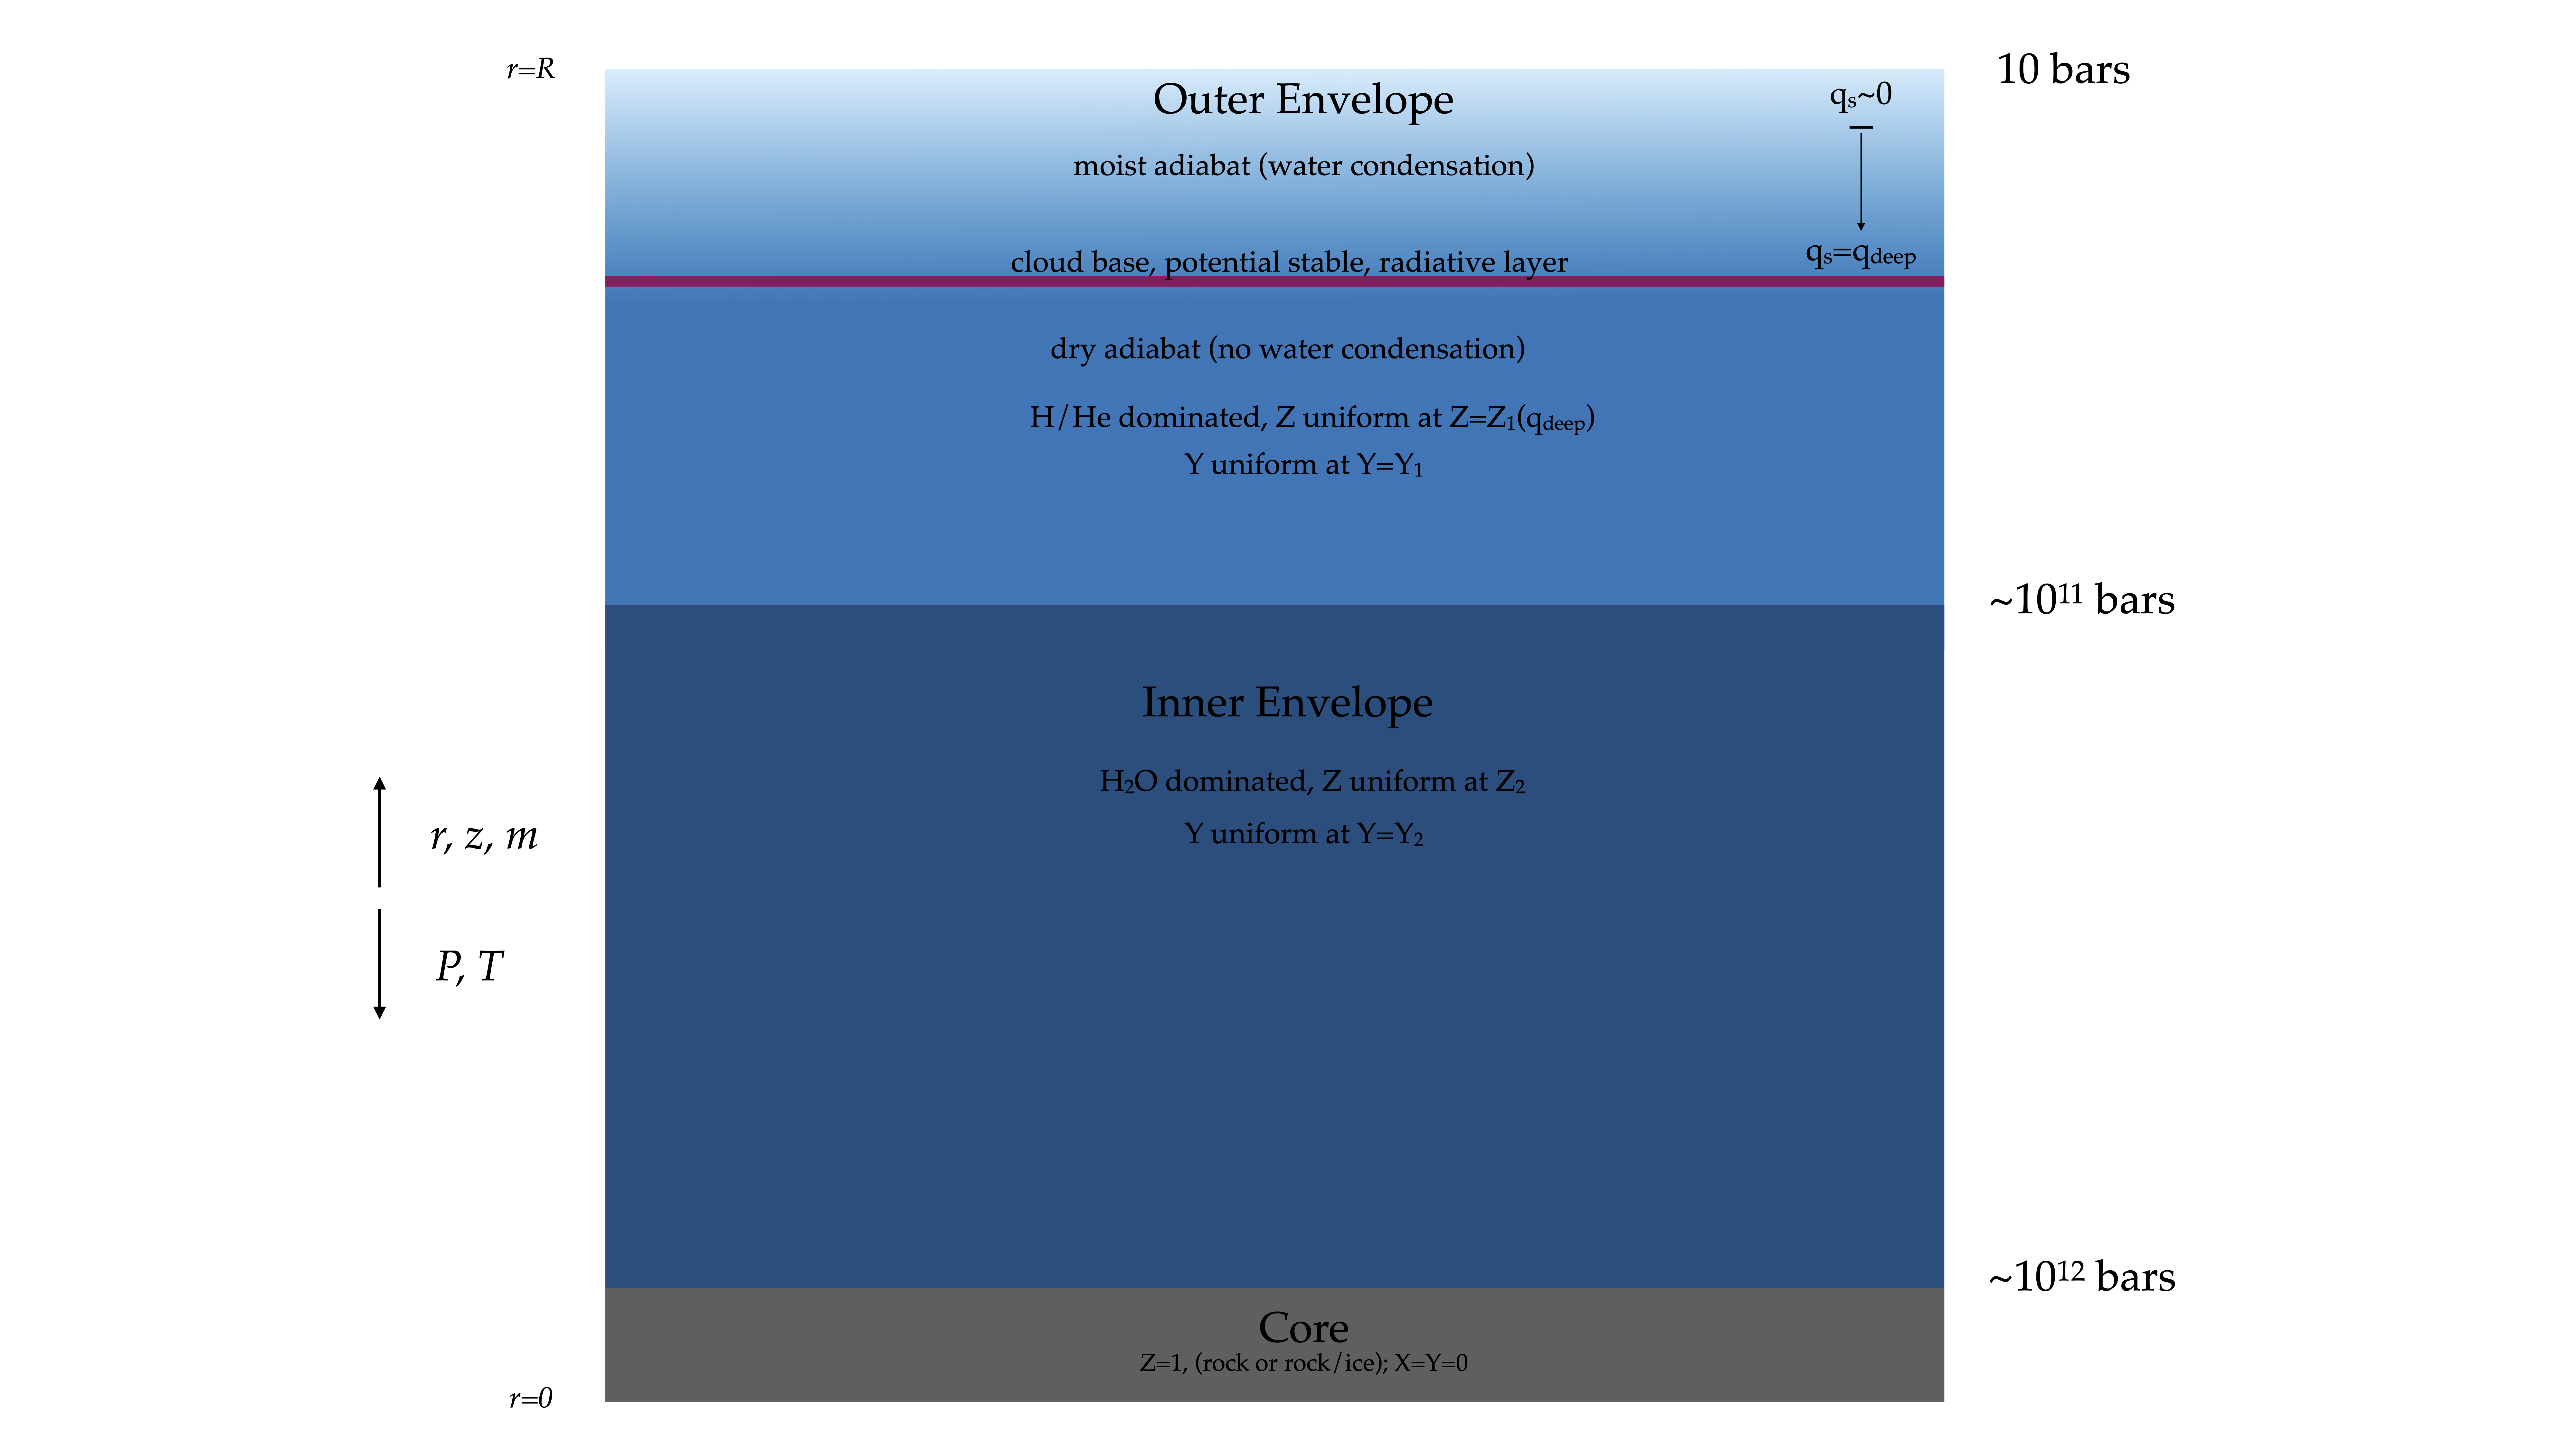
\includegraphics[width=8.0in]{figures/moist_adiabat_structure.png}
 }
\caption[Interior Structure for Moist Adiabat]
{The structure for moist adiabatic interior, allowing for condensation-inhibited convection. In this model, a stable water condensation zone may form. The pressure and temperature at the base of the condensation zone is set by the condition that $x_{\rm vap}$ has reached the deep value $x_{\rm vap}^{\rm deep}$. Below the condensation zone, the temperature and pressure follow a dry adiabat.}
\label{fig:moist_interior}
\end{figure}


\begin{equation}
\nabla_{\rm moist} = (1 + \frac{\frac{x_{\rm vap} L}{R_{\rm gas}T}}{\nabla_{ad} + \frac{L^2}{R_{\rm gas}^2 T^2}} )
\end{equation}
where,
\begin{equation}
\frac{dT}{dP} =\frac{T}{P}\nabla_{\rm moist}
\end{equation}
and the gradient of the water vapor mole fraction \citep{robinson_2016} is given by,
\begin{equation}
\frac{d x_{\rm vap}}{dP} = \frac{x_{\rm vap} L}{R_{\rm gas} T^2} \frac{dT}{dP} - \frac{x_{\rm vap}}{P}
\end{equation}
Gases condense at at sufficiently low temperatures or high pressures. Condensation of a gas is characterized by its saturation vapor pressure, which derives from the Calusius-Clayperon equation \citep{sanchez_2011}. The saturation vapor pressure, $P_{\rm sat}$, is given by: 

\begin{equation}
  P_{\rm sat}(T) = P_{\rm sat}(T_{\rm 0})e^{-\frac{L + C_{\rm p}T_{\rm 0}}{R_{\rm gas}}(\frac{1}{T} - \frac{1}{T_{\rm 0}}) -\frac{C_{\rm p}}{R_{\rm gas}}\ln{\frac{T}{T_{\rm 0}}}}
  \label{eq:saturation_vapor_pressure}
\end{equation}
where $T_{\rm 0} = 273.16K$, and $R_{\rm gas}$ is the gas constant for the condensible species. When the partial pressure of a gas, $P_{\rm gas}$, is less than $P_{\rm sat}$, the parcel of gas is 'unsaturated'. When $P_{\rm gas} = P_{\rm sat}$, the gas is 'saturated'. And, when $P_{\rm gas} > P_{\rm sat}$, the parcel is 'supersaturated'. Every condensible species has its own saturation vapor pressure. 

\begin{figure}[ht!]
 \centerline{
  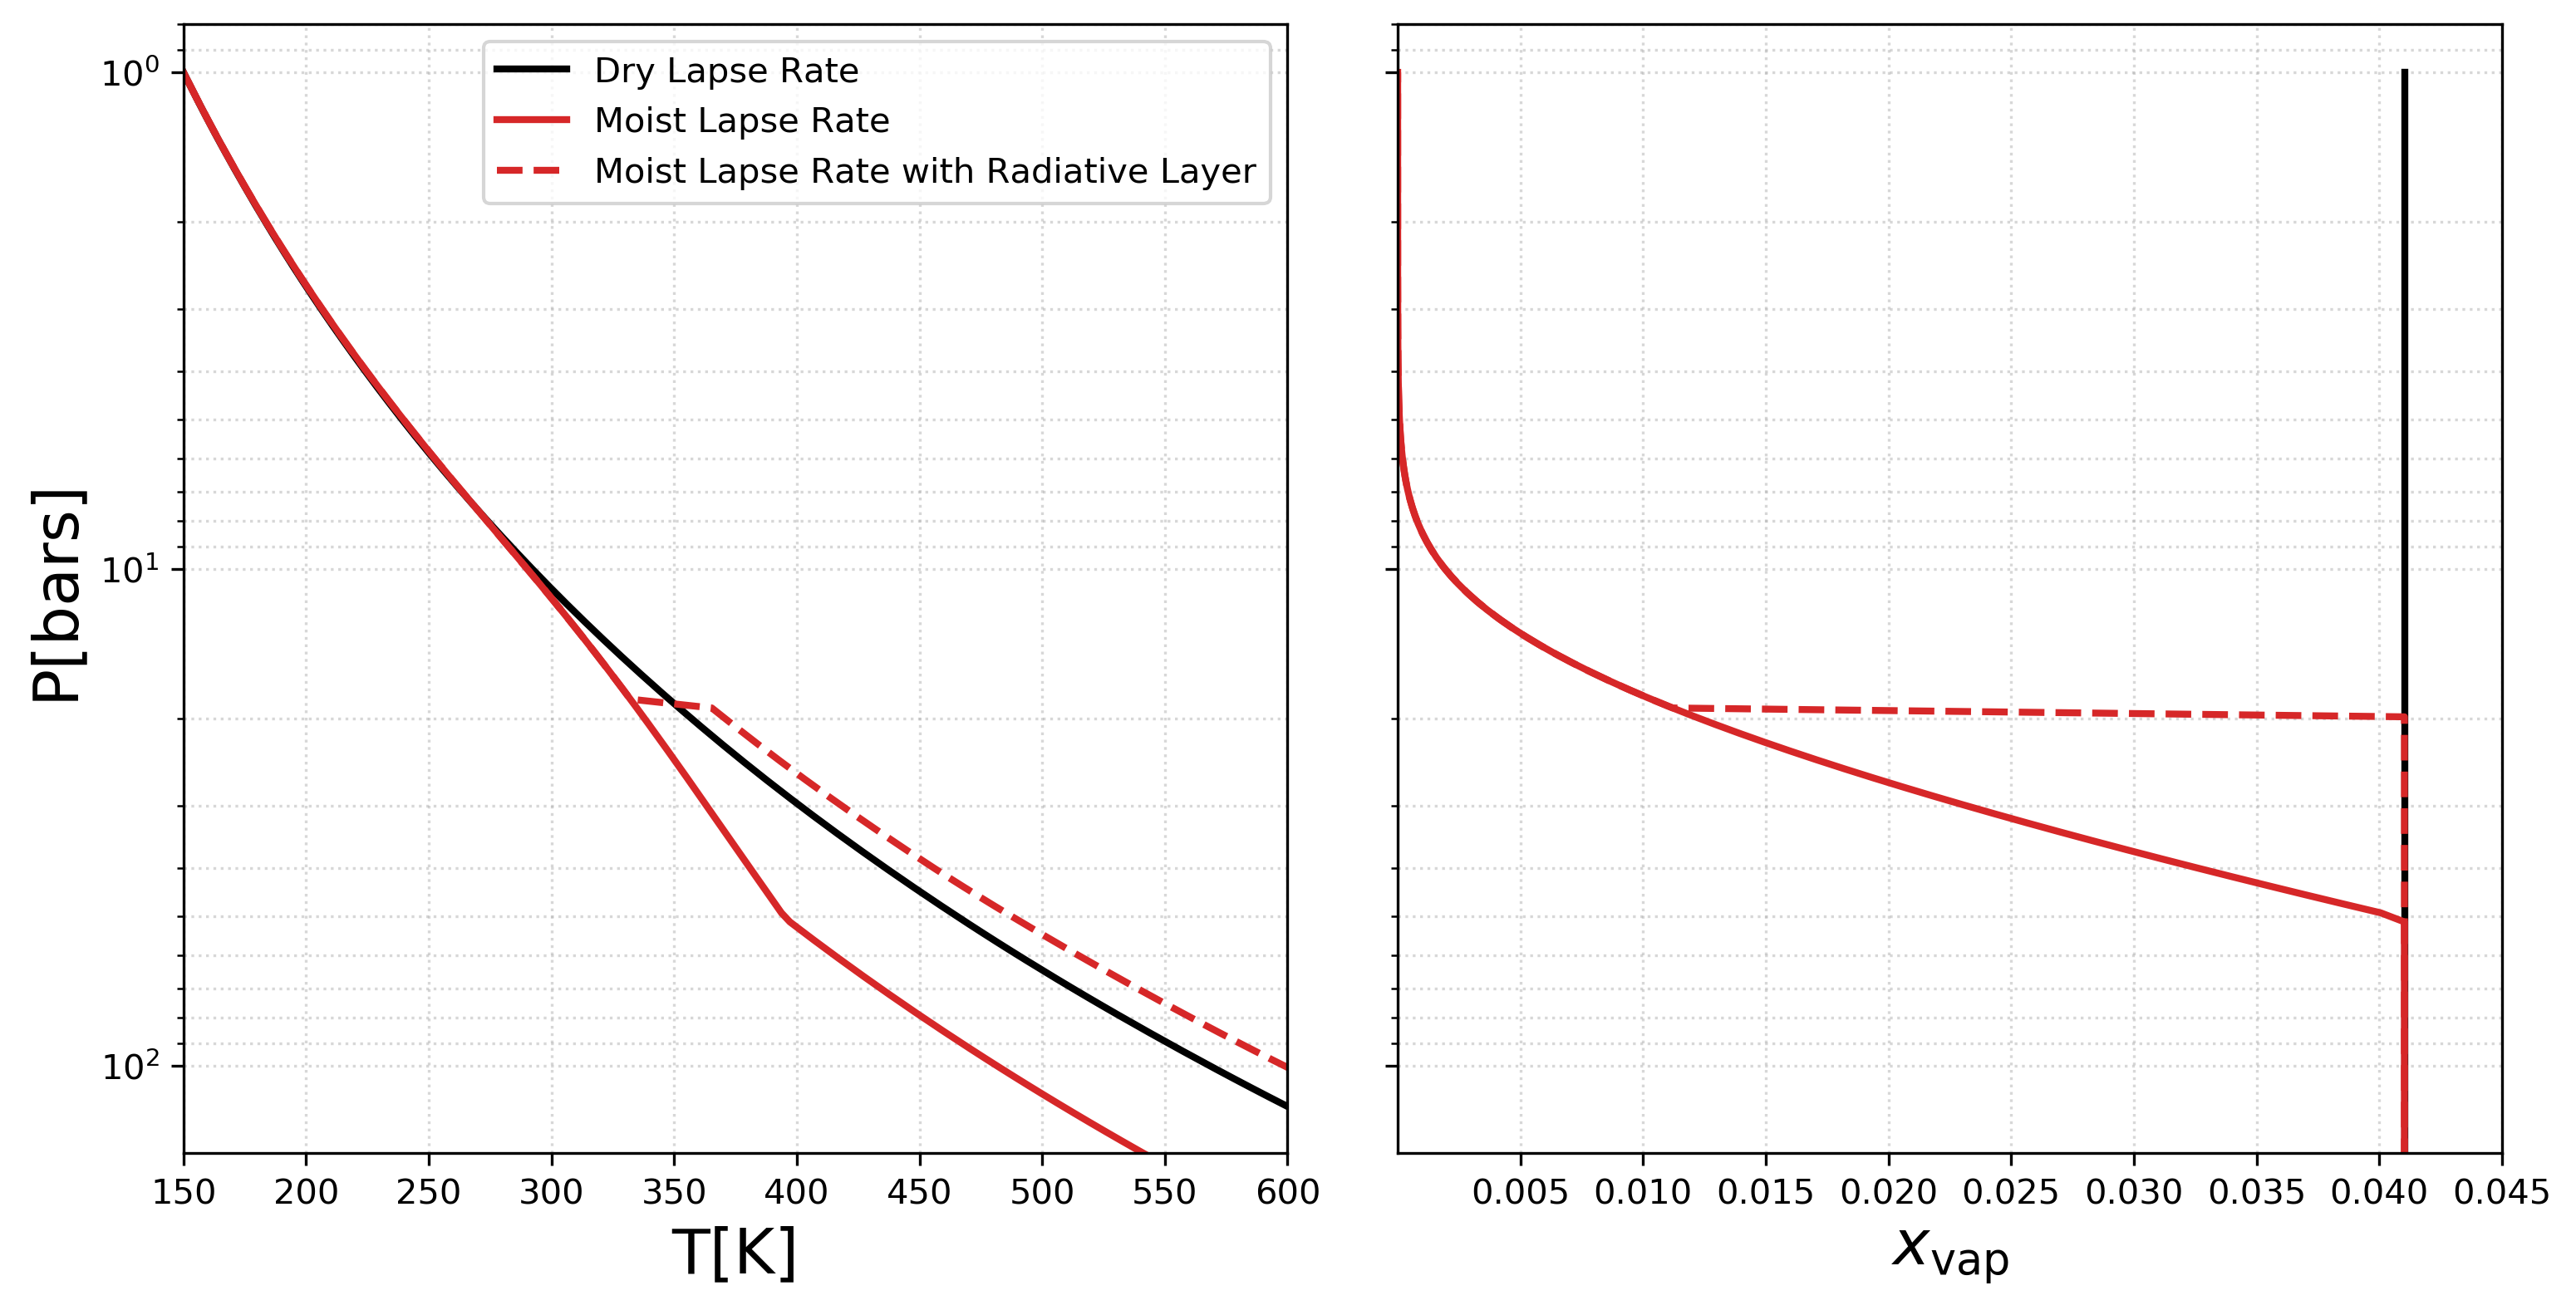
\includegraphics[width=6.5in]{figures/comparison_dry_vs_moist_lapse_rates.png}
 }
\caption[A Standard Interior Structure Model]
{The solid red line is the moist adiabatic lapse rate. The solid black line is the dry lapse rate. The dashed red line is a moist lapse rate with the addition of a stable radiative layer (water condensation zone). The simple moist lapse rate is cooler at depth than either of the other two lapse rates. The presence of a stable radiative layer results in a warmer interiror. These lapse rates assume $q_{\rm deep} = 0.25$ and $T_{1} = 150K$, which is during the period when the onset of condensation-inhibited convection occurs.}
\label{fig:standard_dry_interior}
\end{figure}


If condensation occurs, our model assumes that it may be stable against convection if a fast rainout occurs such that the vertical gradient in mean molecular weight is large enough to counteract the positive bouyancy of the parcel of gas \citep{leconte_2017} \citep{friedson_2017}. In this scenario, condensation-inhibited convection occurs when $\alpha$ is negative, where is $\alpha$ \citep{friedson_2017} is given by:

\begin{equation}
  \alpha = 1 + \xi (q_{s} L / R_{W} T_{0}) 
  \label{eq:alpha}
\end{equation}
where $R_{\rm vap}$ is the gas constant for the vapor (water), $T_{0}$ is the local temperature, $L$ is the latent heat of vaporization for water, $q_{s}$ is the saturation specific humidity, and $\xi$ is given by $\xi = \frac{1}{\epsilon} - 1$, where $\epsilon$ is the ratio of the molecular weight of vapor to the mean molecular weight of dry atmosphere. When $\alpha$ is negative, the vertical gradient in molecular weight results in a stabilizing effect, overwhelming the effects due to latent heat release.

\section{Temperature Jump Across the Water Condensation Zone}
Our model treats the water condensation zone (thin, stable, radiative layer) as a discontinuous increase in temperature. This, thin, stable, radiative layer has a temperature profile that is governed by:

\begin{equation}
  T(P) = T_{\rm top} + \int_{P_{\rm top}}^{P_{\rm base}} \left(\frac{dT}{dP}\right)_{\rm rad}\,d P
  \label{eq:temp_integral_over_radiative_layer}
\end{equation}
with $P_{\rm top}$ and $T_{\rm top}$ denote the pressure and temperature at the top of the stable water condensation zone, and $P_{\rm base}$ represents the bottom of the zone. The integrand in Eqn. ~\ref{eq:temp_integral_over_radiative_layer} is the radiative temprature gradient \citep{leconte_2017}, defined as:
\begin{align}
  \left(\frac{dT}{dP}\right)_{\rm rad}=\frac{T}{P}\nabla_{\rm rad}
  = \frac{T}{P}\times\frac{3}{16}\frac{\kappa_R P}{g}\frac{T_{\rm int}^4}{T^4}
  \label{eq:radiative_gradient}
\end{align}
where $T$ and $P$ are the local temperature and pressure. $T_{\rm int}$ is the intrinsic temperature. The radiative temperature gradient across the water condensation zone is nearly constant, so that Eqn.~\ref{eq:temp_integral_over_radiative_layer} simplifies to:
\begin{align}
T_{\rm base}\equiv T(P+\Delta P) &= T_{\rm top} + \left(\frac{dT}{dP}\right)_{\rm rad}\Delta P
\label{eq:temperature_profile_over_radiative_layer_simplification}
\end{align}
where $\Delta P$ is the extent of the pressure-space of the water condensation zone (radiative layer), given by:
\begin{align}
\Delta P \equiv P_{\rm base}-P_{\rm top} &= \frac{P_{\rm sat}(T_{\rm base})}{x_{\rm vap}^{\rm deep}} - P_{\rm top}.
\label{eq:delta_P_over_radiative_layer}
\end{align}
Within the condensation zone, the vapor mole fraction, $x_{\rm vap}$ is equal to the saturated vapor mole fraction:
\begin{align}
x_{\rm vap}(P, T) &= x_{\rm vap}^{\rm sat}(P, T) = \frac{P_{\rm sat}(T)}{P}, \qquad P<P_{\rm base}.
\label{eq:vapor_mole_fraction_within_condensation_zone}
\end{align}
The base of the condensation zone is set by the condition that $x_{\rm vap}$ has reached the deep value $x_{\rm vap}^{\rm deep}$.
\begin{align}
x_{\rm vap}^{\rm sat}(P_{\rm base}, T_{\rm base}) &= \frac{P_{\rm sat}(T_{\rm base})}{P_{\rm base}}=x_{\rm vap}^{\rm deep}
\end{align}
Below the water condensation zone, the region is subsaturated and hence no condensation occurs. Temperatures below the water condensation zone are obtained by integrating the dry adiabat $\nabla_{\rm ad}$:
\begin{align}
T(P>P_{\rm base}) &= T_{\rm base} + \int_{P_{\rm base}}^P\left(\frac{dT}{dP}\right)_{\rm ad}\,d P
\label{eq:dry_adiabat_integration}
\end{align}


\section{Energy Conservation and Thermal Evolution of Model}
We borrow from conservation of energy and stellar structure and evolution to determine the timestep needed to evolve our model \citep{kippenhahn_2012}. We begin with the planets' intrinsic luminosity, defined as:

[not happy with this section at all.]

\begin{equation}
L_{\rm int} = 4\pi R^2\sigma_{\rm SB}T_{\rm int}^4
\label{eq:intrinsic_luminosity}
\end{equation}
And, the first law of thermodynamics states:
\begin{equation}
dQ = du + Pdv
\label{eq:first_law_thermodynamics}
\end{equation}
where $dQ$ is the heat added per unit mass, $u$ is the internal energy per unit mass, and $v = \frac{1}{\rho}$ per unit mass.
So, for the heat per unit mass shell, we may write:
\begin{equation}
dQ = \big(\epsilon - \frac{dL}{dm})dt
\label{eq:heat_per_unit_mass_shell}
\end{equation}
Substituting our equation for the first law of thermodynamics, we arrive at:
\begin{equation}
\frac{\partial L}{\partial m} = \epsilon - \frac{\partial u}{\partial t} + \frac{P}{\rho^2}\frac{\partial \rho}{\partial t}
\end{equation}
Here, we are not dealing with any nuclear reactions, so $\epsilon = 0$, giving us:
\begin{equation}
\frac{\partial L}{\partial m} = \frac{\partial u}{\partial t} + \frac{P}{\rho^2}\frac{\partial \rho}{\partial t}
\end{equation}



\chapter{Results}

\section{Condensation-inhibited Convection}
We began by looking at if and when condensation-inhibited convection would occur. We ran static models for a variety of $T_{10}$'s, the planet's temperature at $10$ bars. The output of these static simulations are plotted in Figure ~\ref{fig:convection_inhibited}. We ran our model with three different values of $q_{\rm deep}$. The goal was to determine for each deep water concentration, at what pressures and temperatures, condensation-inhibited convection occurs. We find that for $q_{\rm deep} = 0.05$, no condensation-inhibited convection occured. In other words, $\alpha$ (Eqn.~\ref{eq:alpha})  never takes on negative values with this concentration of water vapor, hence the condition for stability is never met. However, for larger values of $q_{\rm deep}$, we find that $\alpha$ does take on negative values (see rows 2 and 3 in Figure ~\ref{fig:convection_inhibited}). The shaded regions of the plots indicate the pressure-space over which $\alpha$ is negative. We show $\alpha$ with respect to pressure, vapor mole fraction, and temperature. Note: the top of the shaded region in each plot indicates where the base of the condensation zone forms. [not sure if i should go into the issue of the reainder of the shaded region having no physical meaning]. Looking at these plots, for $q_{\rm deep} = 0.15$ and $q_{\rm deep} = 0.25$, we can see that condensation inhibited convection sets in at approximately $T_{10} = 335K$. Note: The $T_{10}$ at which the onset of condesation occurs is dependent on the resolution of the simulation. As such, these plots are meant to show the likelehood of condensation-inhibited convection rather than the exact moment or specific deep water concentration for which it occurs. [I'm not very happy with the results section so far]

\begin{figure}[ht!]
 \centerline{
  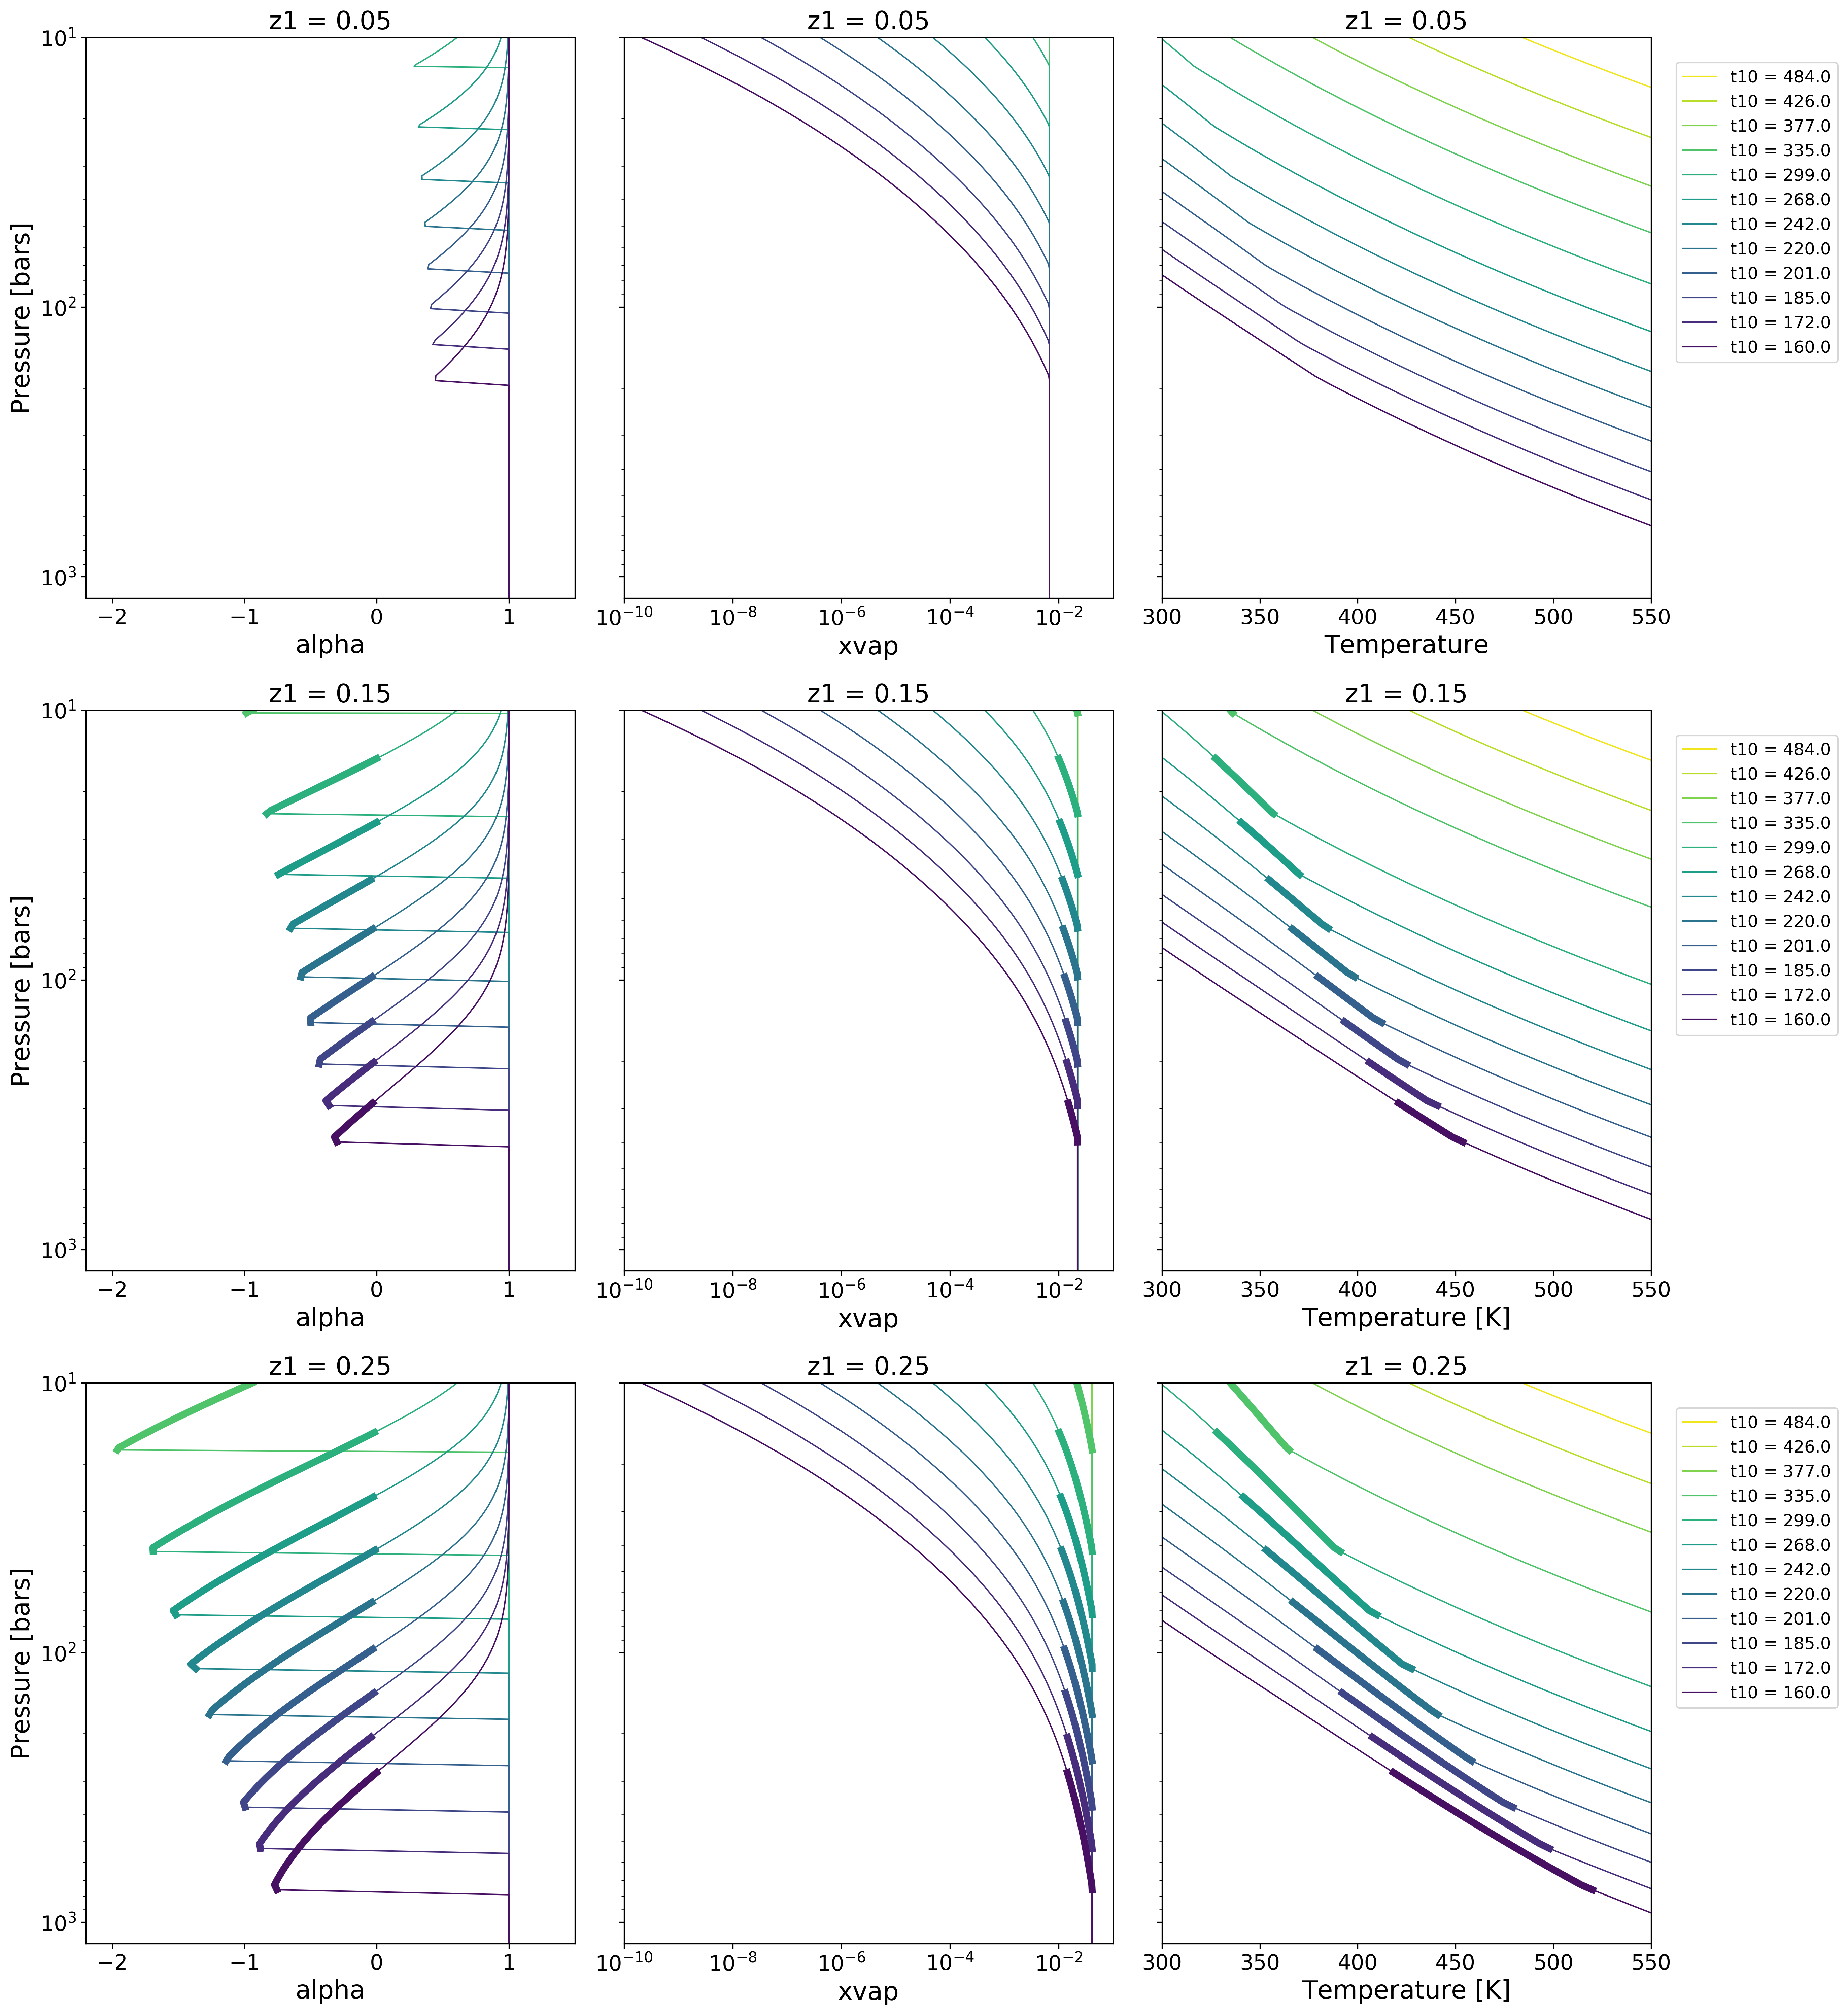
\includegraphics[scale=0.36]{figures/convection_inhibited_2.png}
 }
\caption[Inhibition of convection on Uranus]
{Each row represents a different value for $q_{\rm deep}$. For the top row, $q_{\rm deep} = 0.05$, for which no stable condensation zone forms. For the the moddle row, $q_{\rm deep} = 0.15$, and for the third row $q_{\rm deep} = 0.25$. For thee concentrations, stable condensation zones can form. The shaded regions of the plots indicate zones where $\alpha$ is negative, or where stable zones can form.}
\label{fig:convection_inhibited}
\end{figure}


\section{Formation of Radiative Zone}
The plots in Figure~\ref{fig:radiative} show the lapse rate (first column), and the change in the vapor mole fraction for $H_{2}O$ (second column), for three different values of $q_{\rm deep}$, $0.05$, $0.15$, and $0.25$, for rows 1 through 3, respectively. In the first row, we can see that for early $T_{10}$'s, there is no onset of condensation, and the lapse rate follows a dry adiabat. For later $T_{10}$'s, there is a visible kink in the lapse rate which indicates the onset of condensation, at which point the lapse rate has a shallower slope. For the larger values of $q_{\rm deep}$, where $\alpha$ takes on negative values, we see the onset of condensation-inhibited convection and the establishment of a radiative zone. In the plots, the water condensation zones are represented by the horizontal discontinuites moving from left to right. As the planet cools, these radiative zones descend deeper into the planet's interior. When the radiative zones are established, the interiror below the zone warms. Looking at Figure~\ref{fig:overlay}, we have overlayed the lapse rate for $q_{\rm deep} = 0.25$ (exhibiting stable water condensation zones) over the lapse rate for $q_{\rm deep}=0.05$ (no stable zones). From this plot, one can see that the presence of a radiative zone creates a tempearure jump such that a given $T_{10}$ appears to look like an earlier $T_{10}$. In other words, in the presence of radiative zones, the interiror appears as warm as an interiror described by an earlier $T_{10}$. [ugh. gotta be a better way to describe this]

\begin{figure}[ht]
 \centerline{
  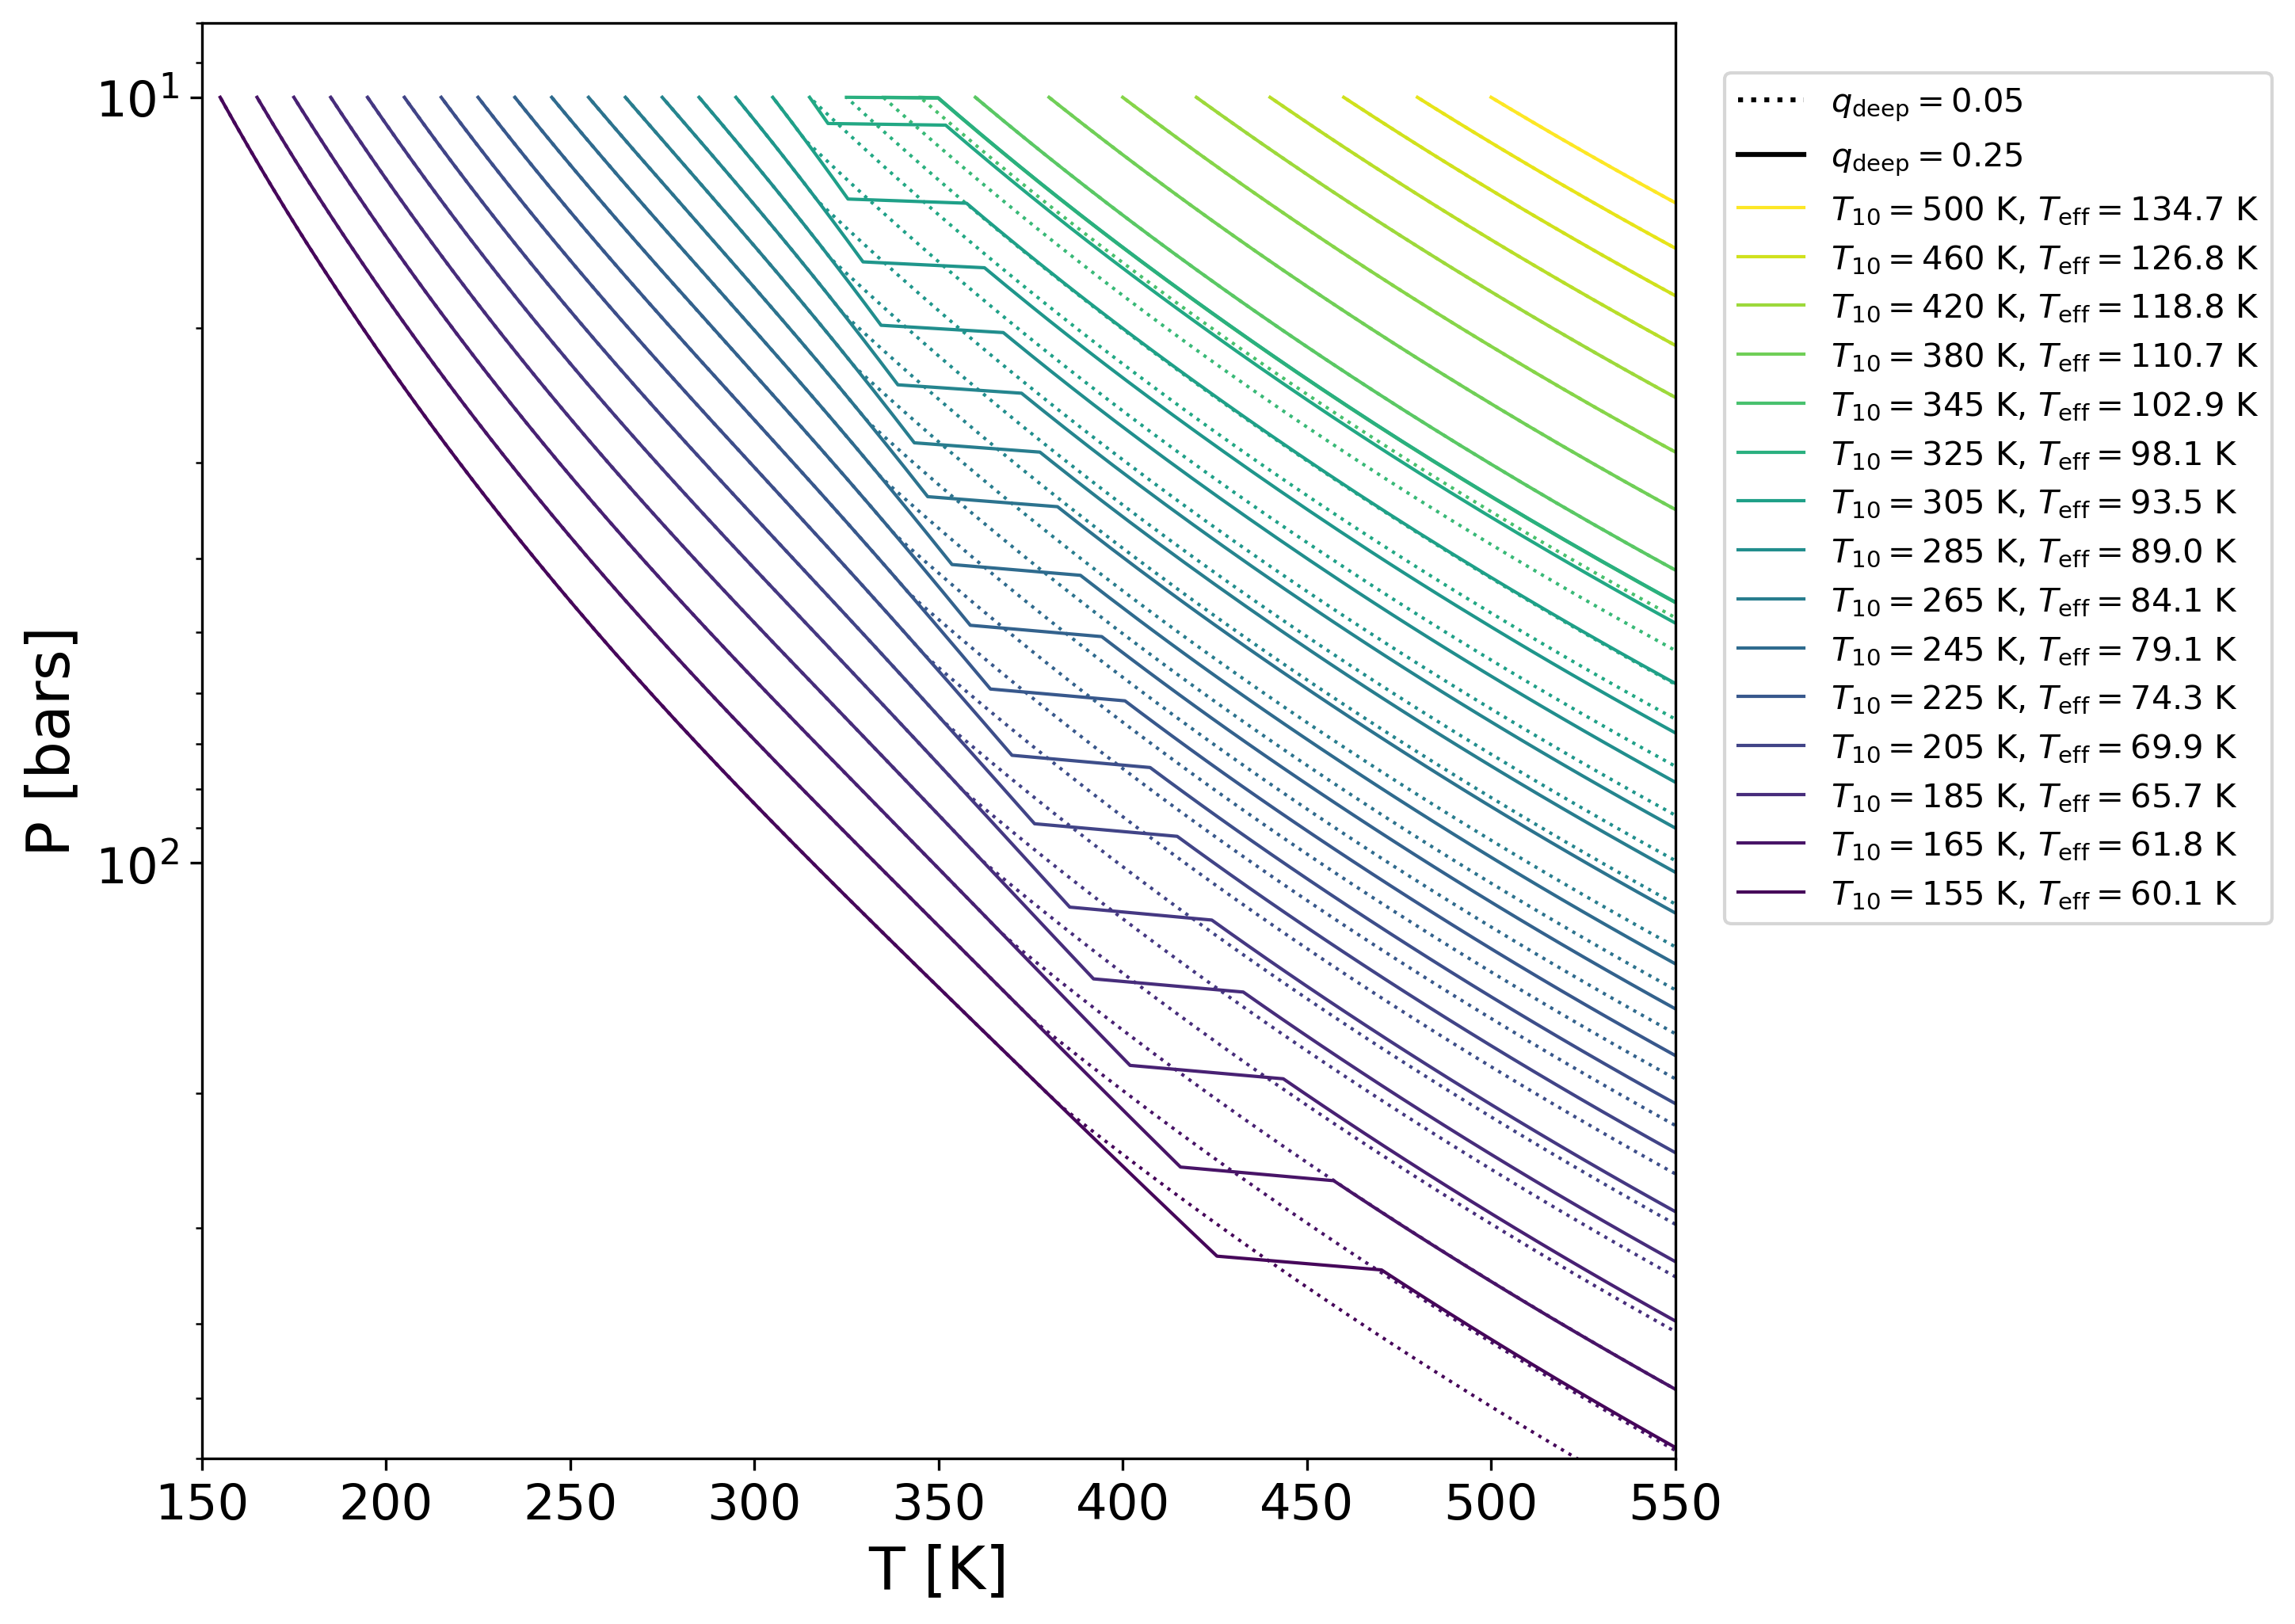
\includegraphics[scale=0.7]{figures/thesis_static_radiative_layer_plot_diff_qdeep_overlay.png}
 }
\caption[Impact of Radiative Layer on T10]
{The solid lines represent the lapse rate for $q_{\rm deep} = 0.25$, and the dashed lines for $q_{\rm deep}=0.05$. Looking at recent $T_{10}$'s, the lapse interiror temperature for $q_{\rm deep} = 0.25$ jumps to an earlier $t_{10}$. The radiative layer traps heat, such that the interiror looks like the interiror from an earlier $T_{10}$.}
\label{fig:overlay}
\end{figure}

Looking at the adjacent $x_{\rm vap}$ plots, we can see that $x_{\rm vap}$ follows its saturated value. At the bootom of the radiative zone, the vapor mole fraction equals its deep water value, which sets the conditions for the creation of the base of the condensation zone. 

\begin{figure}[ht]
 \centerline{
  \includegraphics[scale=0.3]{figures/thesis_static_radiative_layer_plots_without_grid_points.png}
 }
\caption[Formation of Radiative Zone]
{These plots were generated using our model Uranus. Again, from top to bottom row, we move from $q_{\rm deep} = 0.05$, $0.15$, and $0.25$, respectively. $T_{10}$'s range from hotter (yellow) to cooler (purple), more recent temperatures. In the top row, no stable radiative zones are formed. The kink visible in the middle of the top left plot represents the transition from a moist to dry adiabat. Condensation occurs, but no stability is achieved. In rows two and three, stable radiative zones are formed, as indicated by the discontinuous temperature jumps moving left to right. The radiative zones form deeper in the interiror as the planet cools. The plots in the second column show the vapor mole fraction with respect to pressure. The vapor mole fraction is constant within the radiative zone and reaches its deep water concentration value at the bottom of the radiative zone. }
\label{fig:radiative}
\end{figure}


\section{Thermal Evolution of Uranus and Neptune}

% cooling camparisons of dry adiabat, moist adiabat, and moist adiabat with radiative layer
We simulated the thermal evolution of Uranus and Neptune using a variety of variety of input parameters. In Figure~\ref{fig:evolve_adiabats}, we display the results of evolutionary tracks  that considered separately the evolution of a dry adiabat, a moist adiabat with condensation but no stable radiative zone, and a moist adiabat with condensation containing stable radiative zones. For all of these evolutionary tracks, we assumed $q_{\rm deep} = 0.25$. Looking at these evolutionary tracks, the coolest scenario at present time, is a moist adiabat that is never stable against convection. The moist adiabat that is stable against convection has the warmest outcome at present time. In Figure~\ref{fig:evolve_uranus_qdeeps} and Figure ~\ref{fig:evolve_neptune_qdeeps}, we consider the impact of different deep water concentrations on the thermal evolution of Uranus and Neptune, respectively. As the planets cool, their radiative zones descend deeper into the interiror, as we saw in Figure~\ref{fig:radiative}. This feature is also noticable in the thermal evolution plots. Looking at $T_{\rm eff}$ at ~$7 \times 10^7$ Gyr, the onset of condensation-inhibited convection occurs, resulting in a discontinuous temperature drop. The same behavior is seen in the $T_{10}$ plot, however, by this time the radiative zone has descended deeper, later in time at around ~$7 \times 10^8$ Gyr. Larger $q_{\rm deep}$'s result in warmer Uranus and Neptune at present time. We also look at the impact of $q_{\rm deep}$ on the evolution of planetary radius and find that larger values of $q_{\rm deep}$ tend to converge more closely toward the presntly observed radius for both Uranus and Neptune in these simulations. [needs more work]

\begin{figure}[ht]
 \centerline{
  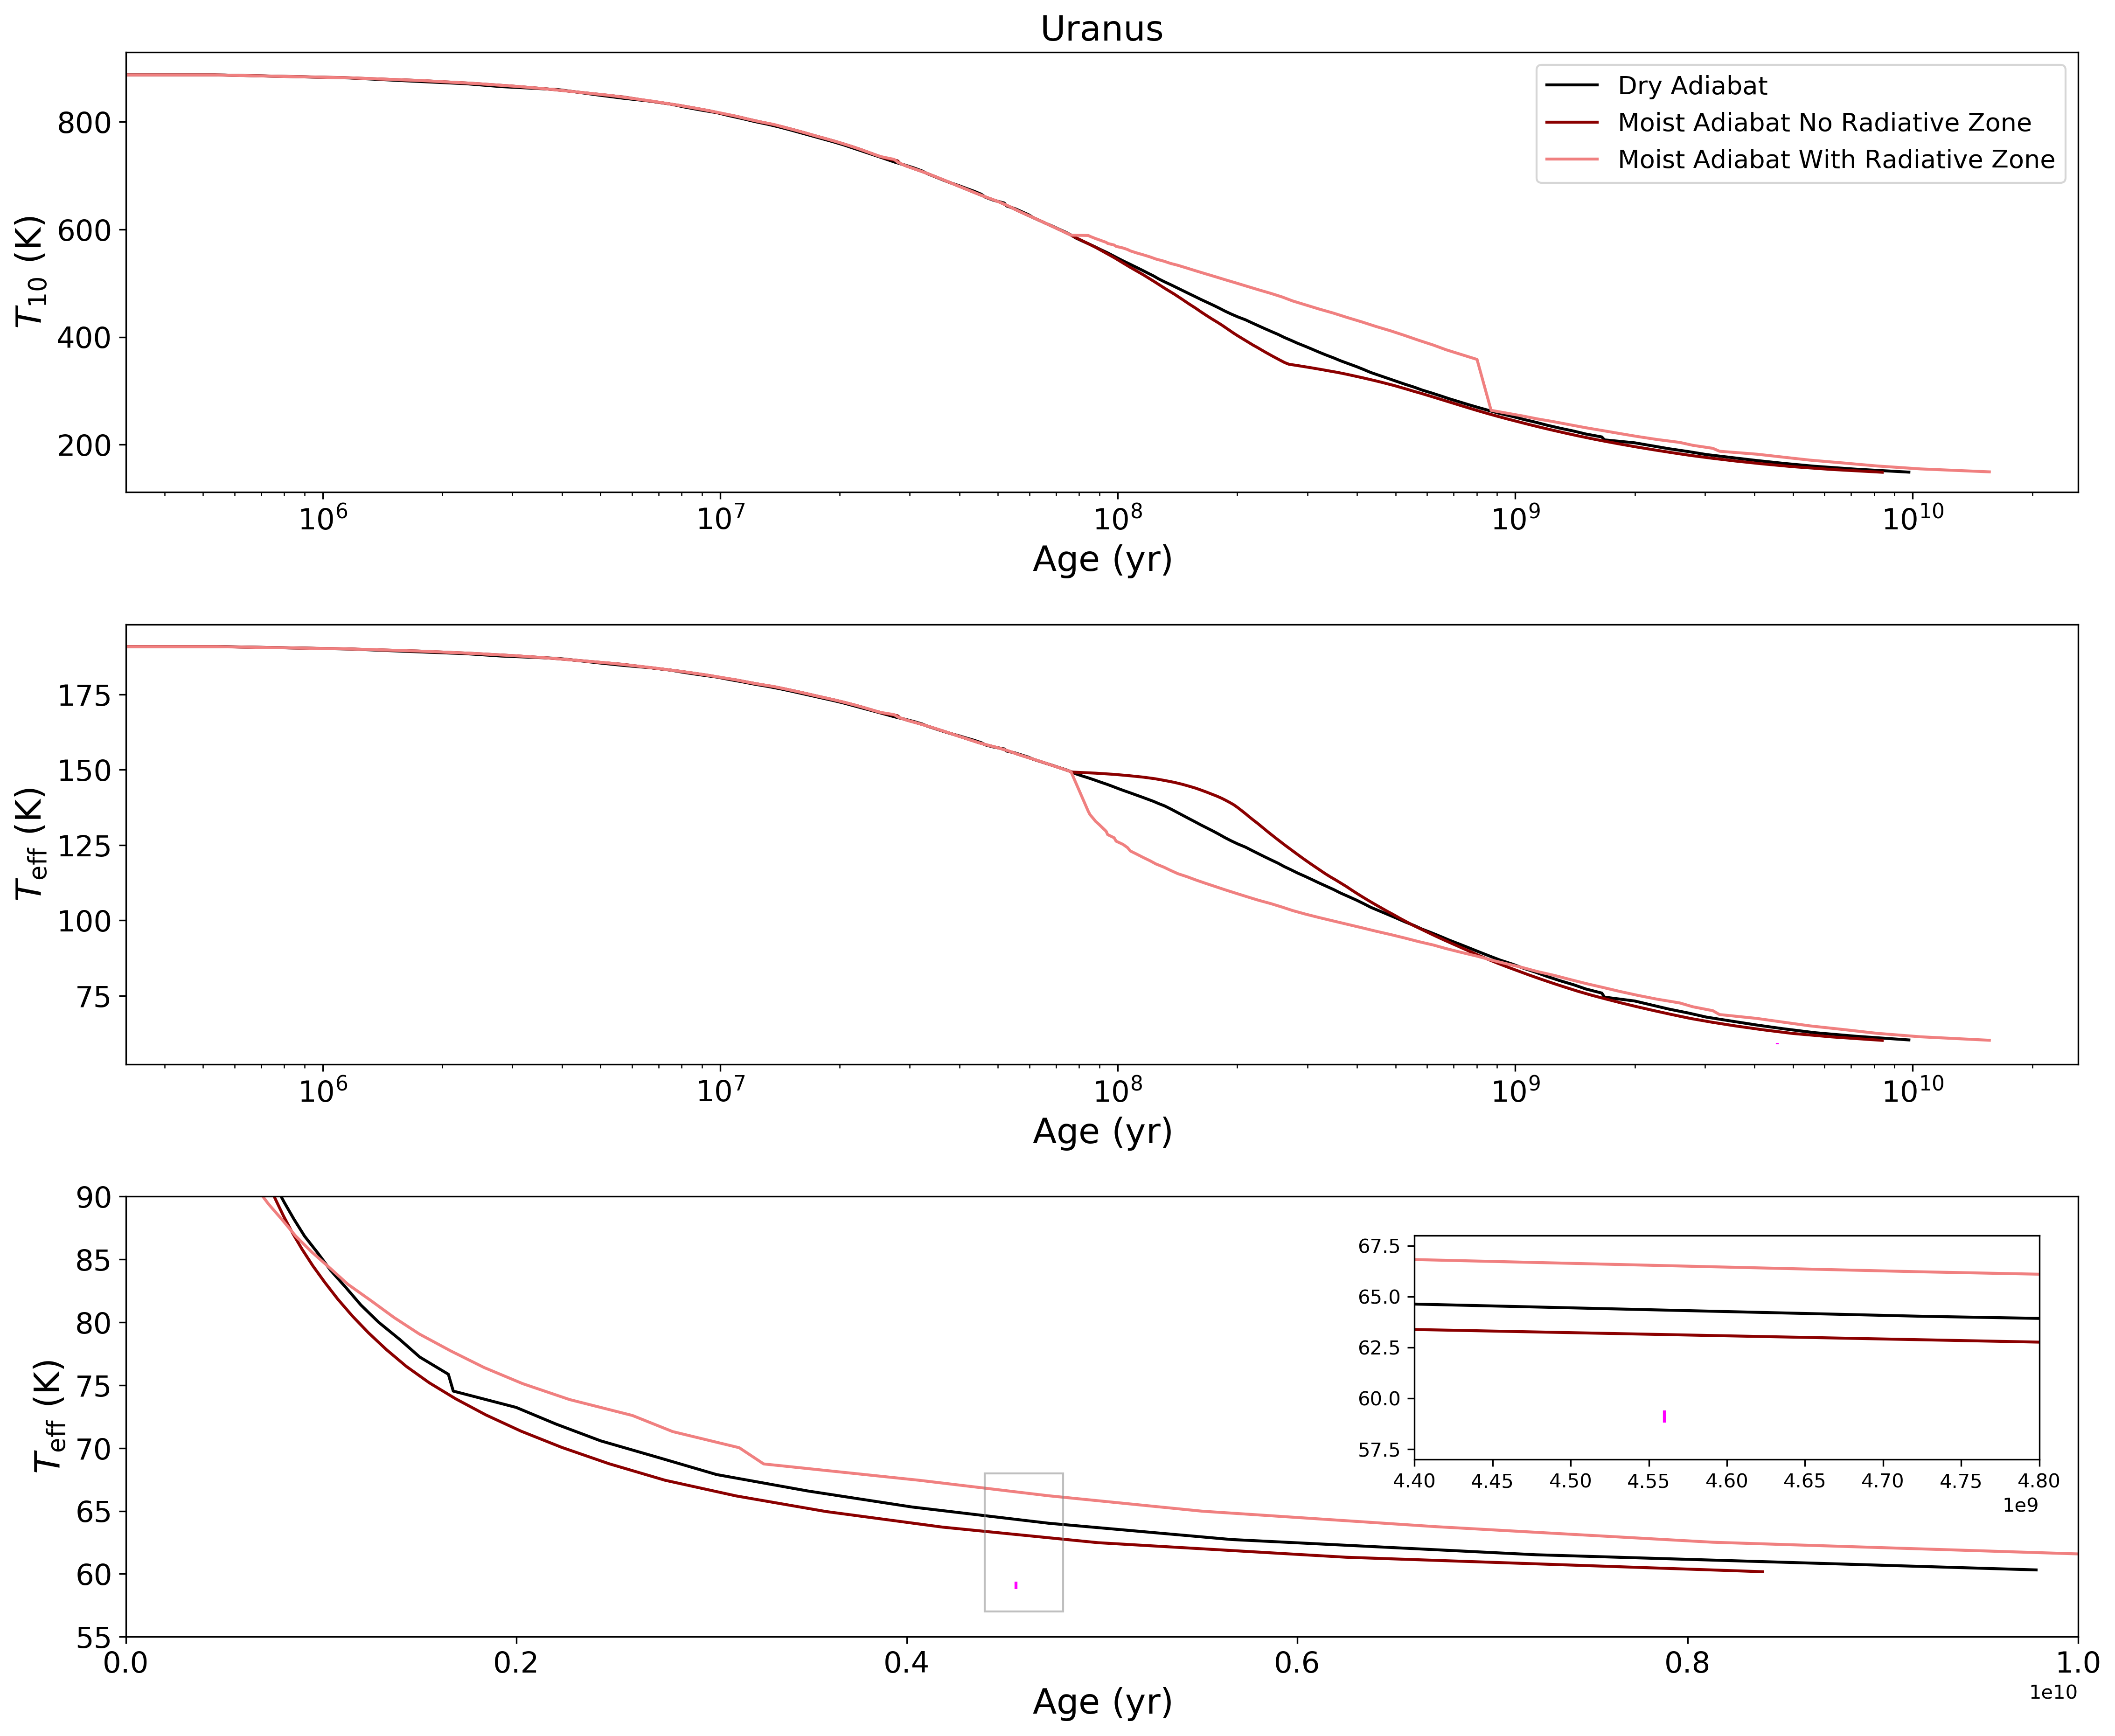
\includegraphics[scale=0.5]{figures/dry_moist_radiative_u_cooling_curves_adiabat_comparisons.png}
 }
\caption[Thermal Evolution Curves for Uranus - Adiabat Comparisons]
{The black line represents the thermal evolution for a dry adiabat. The dark red line represents the thermal evolution for a moist adiabat that does not allow for the formation of a stable radiative layer. The light red line represents the thermal evolution of a moist adiabat that does allow for the formation of a stable radiative zone. The fuschia dot on the lower plot represent the currently observed effective temperature of Uranus[include temp], plus or minus [include temp error]. }
\label{fig:evolve_adiabats}
\end{figure}

% cooling uranus
\begin{figure}[ht]
 \centerline{
  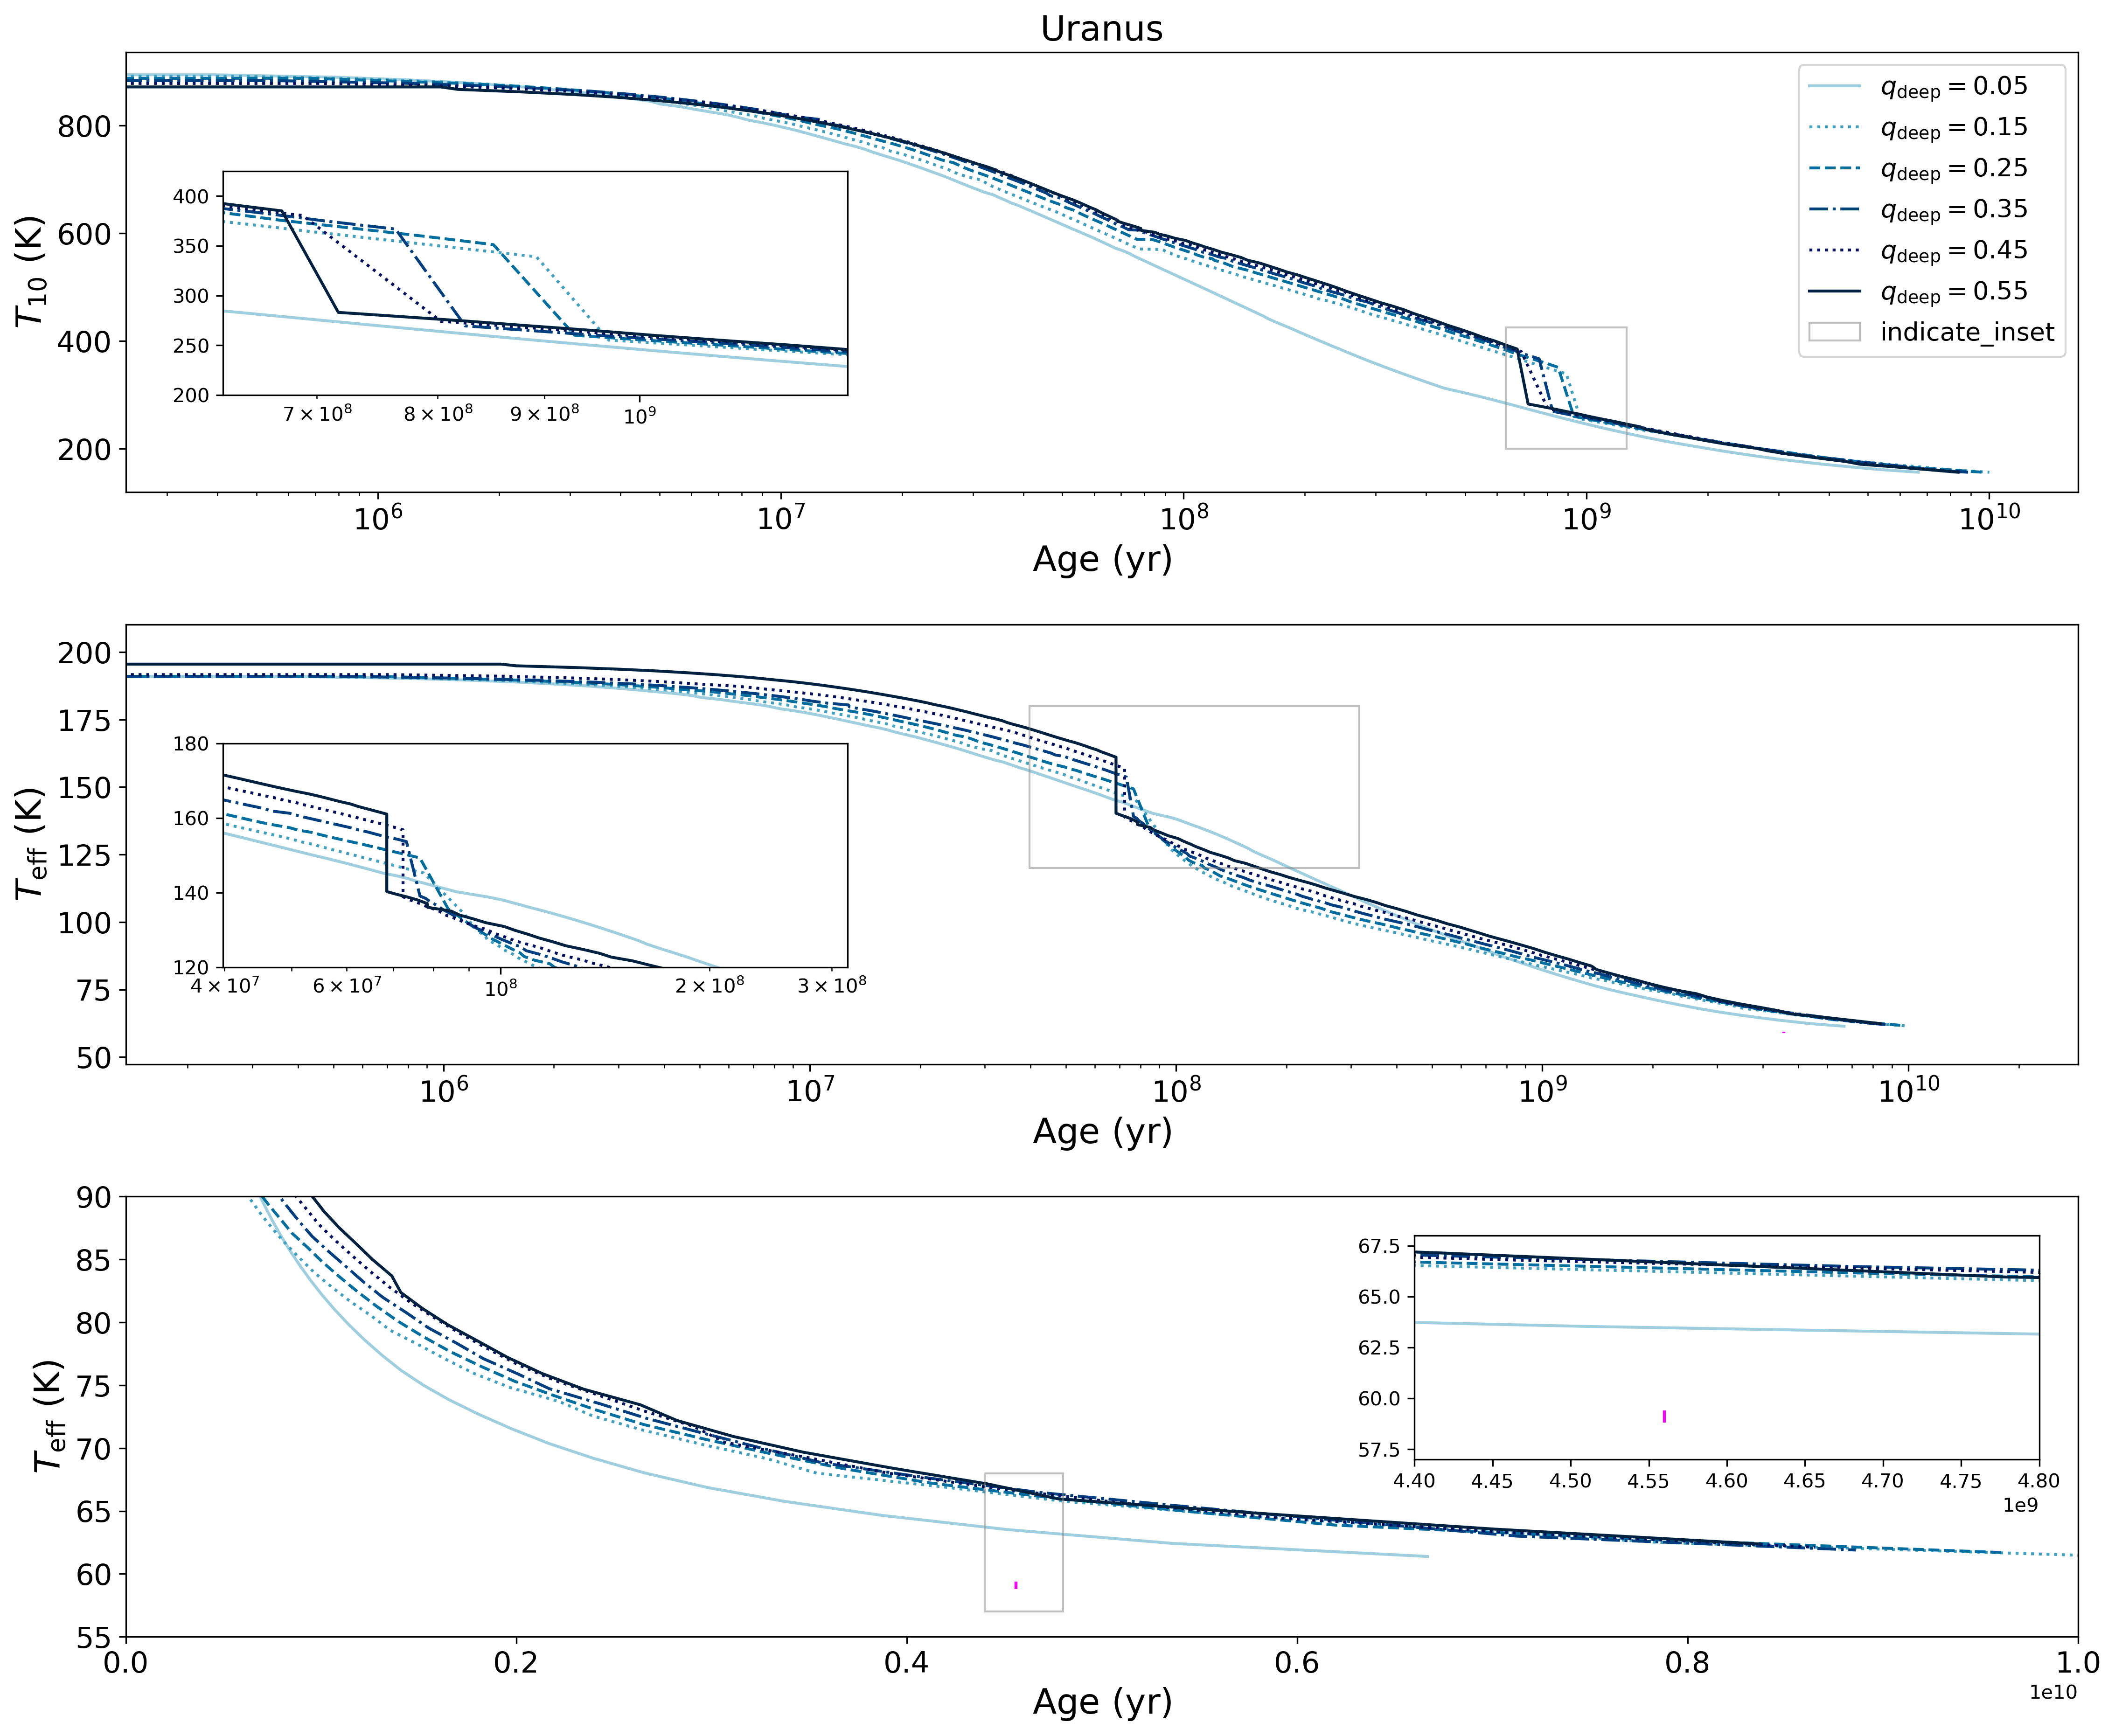
\includegraphics[scale=0.45]{figures/u_cooling_curves_nz_4096_more_qdeeps.png}
 }
\caption[Thermal Evolution Curves for Uranus - Water Vapor Concentration Comparisons]
{The curves in these plots represent thermal evolution tracks for different values of $q_{\rm deep}$. Dark blue is the largest concentration of water vapor, at $q_{\rm deep} = 0.55$ and the light blue line is the least concentration of water vapor at $q_{\rm deep} = 0.05$. For $q_{\rm deep} = 0.05$, there is no onset of condensation-inhibited convection and no rapid cooling episode. For larger values of $q_{\rm deep}$ there is a rapid cooling episode for $T_{\rm eff}$ at around $10^8$ Gyr. Similarly, a rapid cooling episode is visible deeper down in the interior as seen in the $T_{10}$ curves at around $10^9$ Gyr. }
\label{fig:evolve_uranus_qdeeps}
\end{figure}

%  cooling neptune
 

\begin{figure}[ht]
 \centerline{
  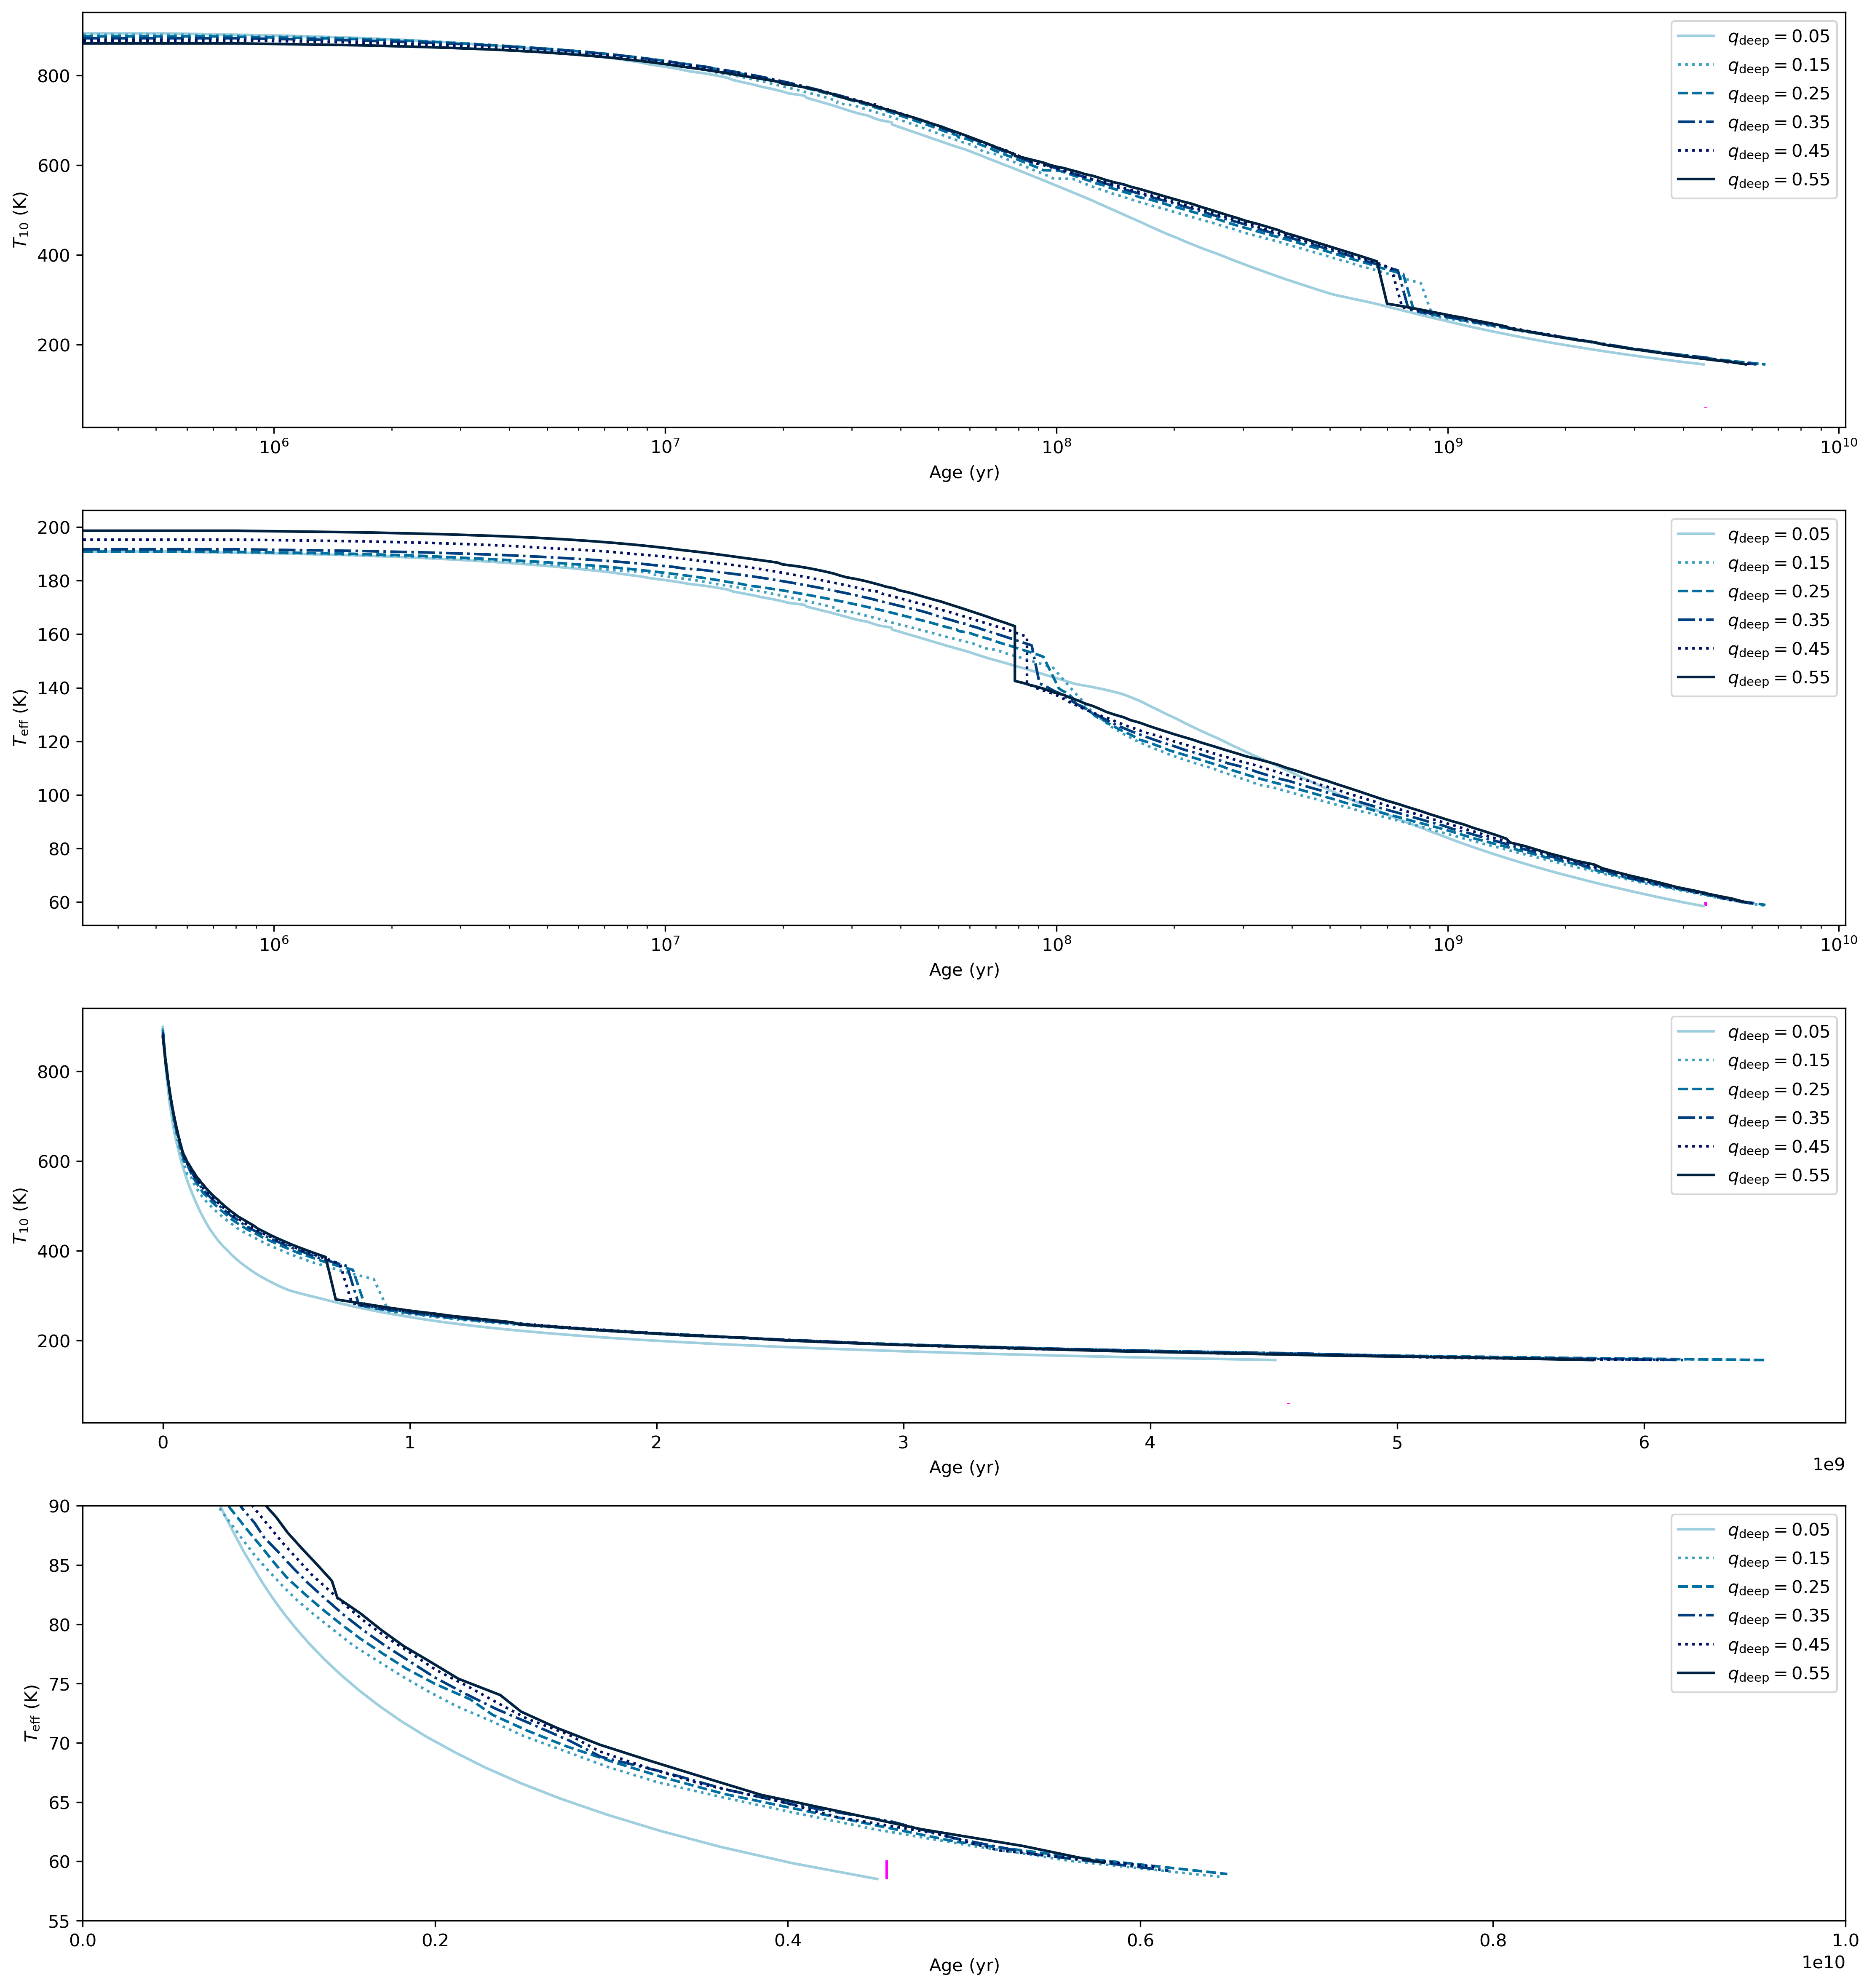
\includegraphics[scale=0.45]{figures/n_cooling_curves_nz_4096_more_qdeeps.png}
 }
\caption[Thermal Evolution Curves for Neptune - Water Vapor Concentration Comparisons]
{Similar to the Uranus plots, these curves represent cooling tracks for $q_{\rm deep}$'s ranging from $0.05$ to $0.55$. Similar to Uranus, the rapid cooling episodes for $T_{\rm eff}$ and $T_{10}$ occur at $10^8$ Gyr and $10^9$ Gyr, respectively. The vertical fucshia line in the bottom plot indicates the current observed effective temperature of Neptune [include temp], plus or minus [include temp error] }
\label{fig:evolve_neptune_qdeeps}
\end{figure}



%  cooling radius curves
\begin{figure}[ht]
 \centerline{
  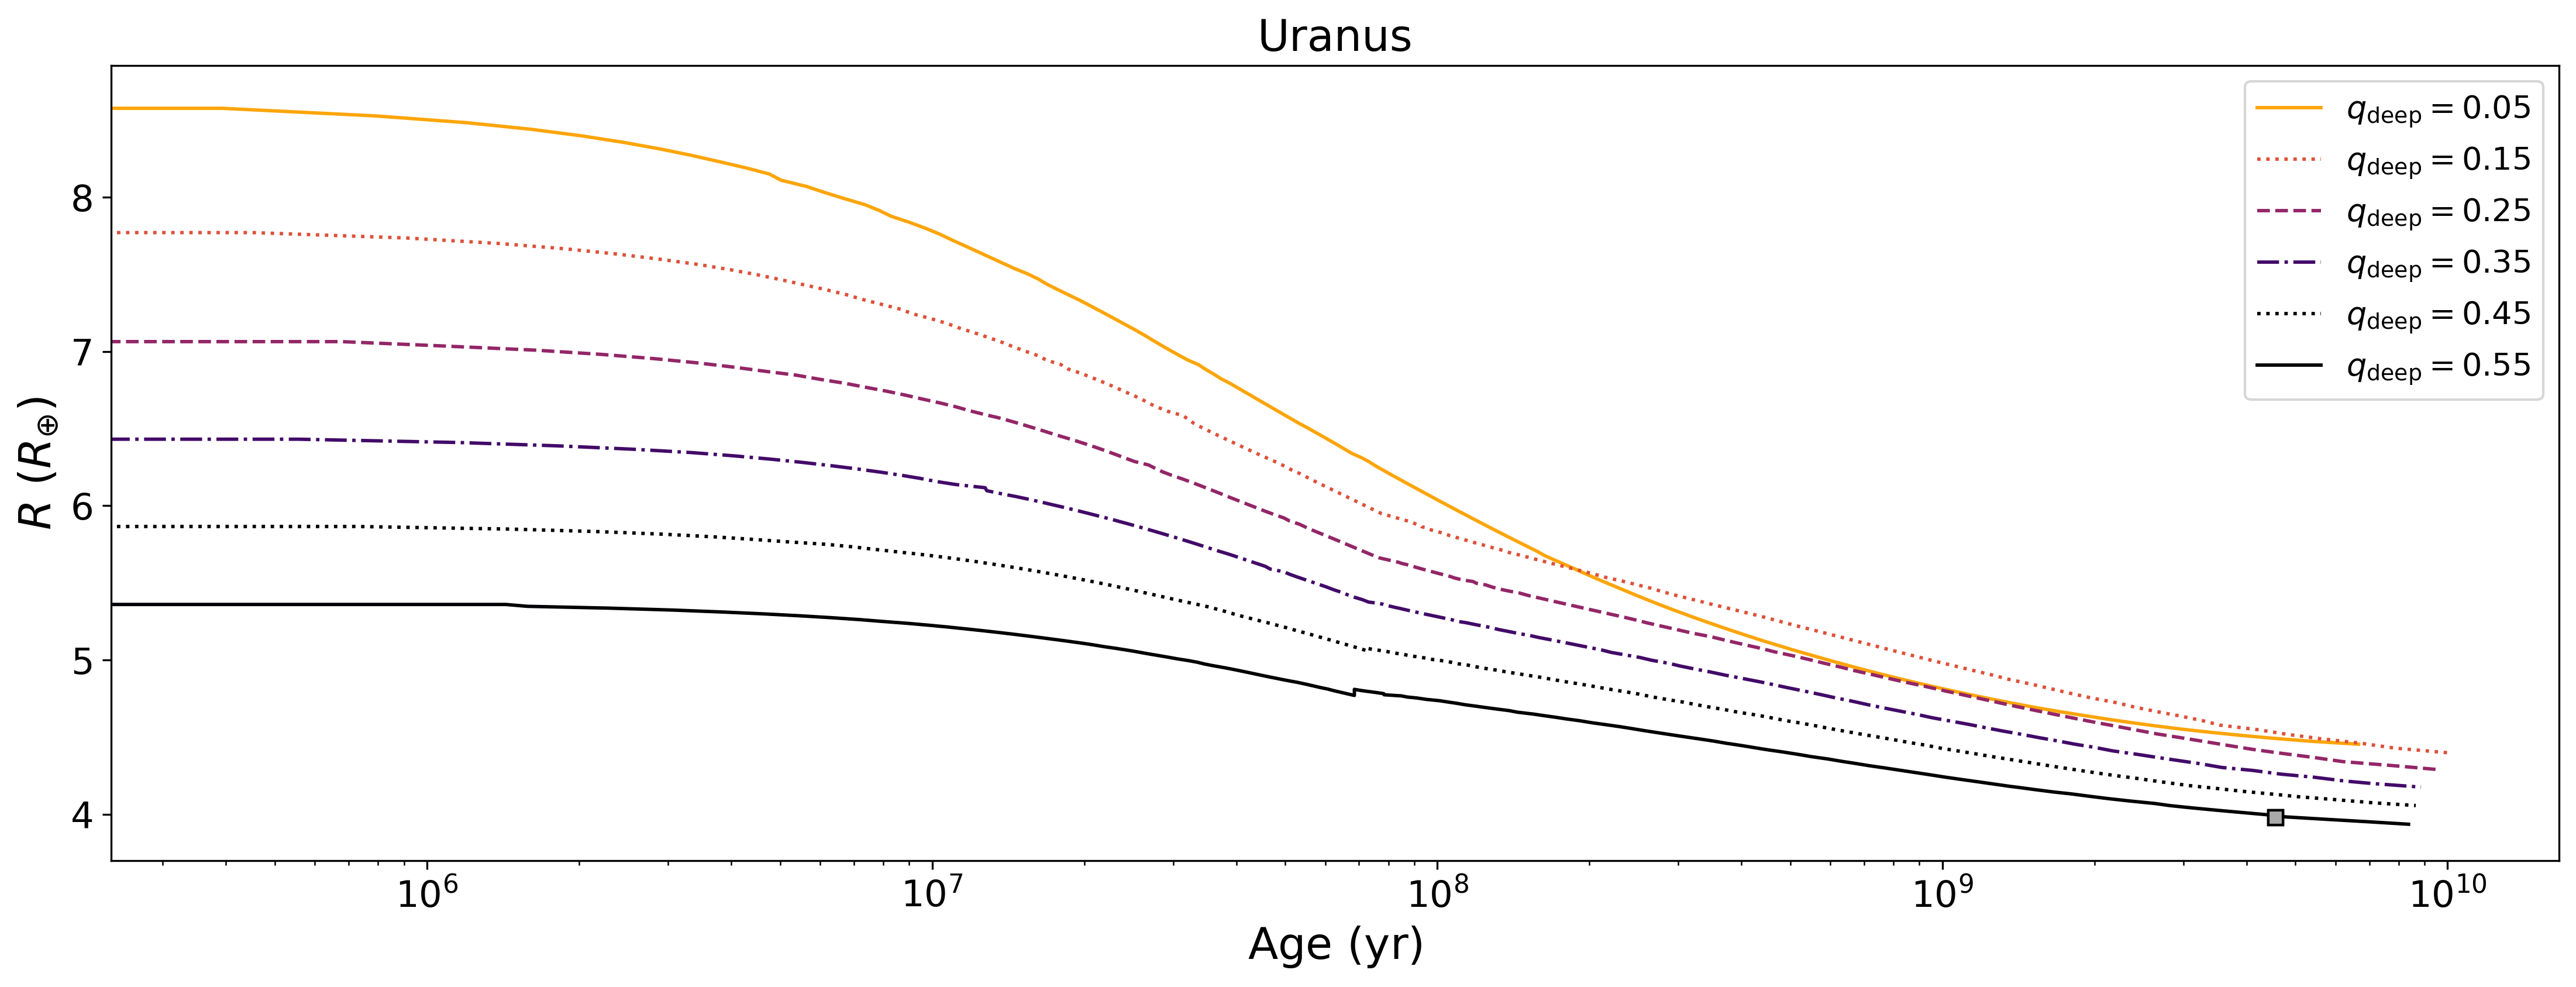
\includegraphics[scale=0.45]{figures/u_cooling_radius_nz_4096_logx_more_qdeeps.png}
 }
\caption[Thermal Evolution Curves for Uranus - Radius]
{This thermal evolution plot shows the impact of different deep water concentration on the radius as the planet cools. The gray square represents the current observed radius.}
\label{fig:evolve_uranus_radius}
\end{figure}


\begin{figure}[ht]
 \centerline{
  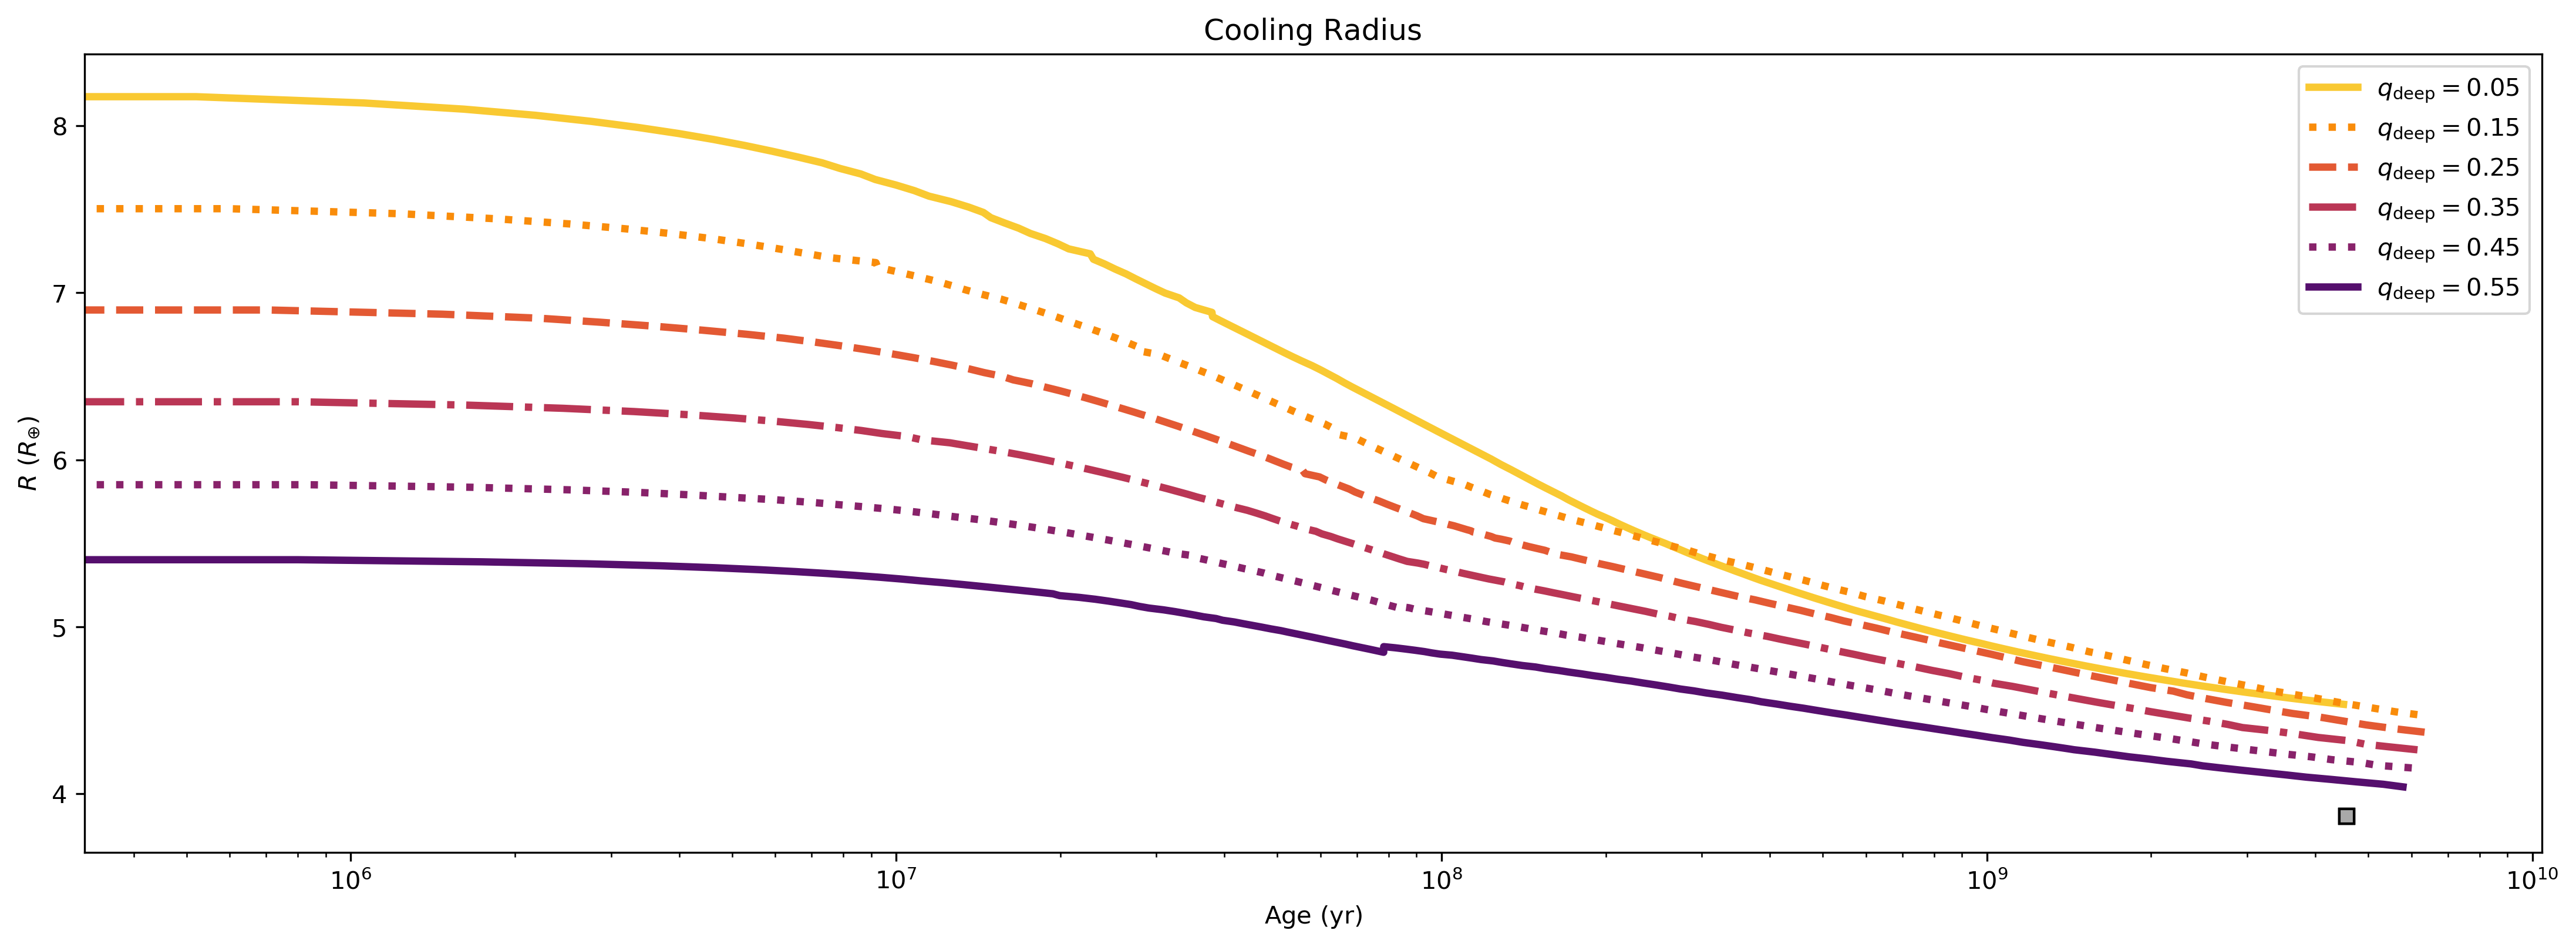
\includegraphics[scale=0.45]{figures/n_cooling_radius_nz_4096_logx.png}
 }
\caption[Thermal Evolution Curves for Neptune - Radius]
{[Combine this plot with the above and have one caption.] }
\label{fig:evolve_neptune_radius}
\end{figure}



\chapter{Discussion and Conclusions}
[I wrote this just before sending. i'm sure I'll want to make changes when i re-read in the morning]
We set out to investigate the impact of water condensation zones on the thermal evolution of our solar system ice giants. It has been speculated that such thermal boundary layers could act as an imperfect insulator, trapping heat below and allowing the envelope above the boundary layer to cool more rapidly \citep{nettelmann_2016}\citep{friedson_2017}\citep{leconte_2017}\citep{podolak_1991}\citep{scheibe_2019}. It seems plausible that interirors containing these thermal boundary layers could explain the problem with Uranus appearing to have no intrinsic temperature. Our findings are inconclusive. We do find that incorporating a moist adiabat into our interiror structure model does result in a cooler planet than would otherwise be seen with a purely dry model. However, when we add stable radiative zones to the interior, we do find in the planet's past a period of rapid cooling that results in a cooler effective temperature at around $10^8$ Gyr, the planet eventually becomes warmer at present time than predicted by dry or simple moist adiabatic models. Reality is certainly more complex than the assumptions upon which our model is based. It is quite possible that reality resembles something in between the binary choice of a moist adiabat with or without thermal boundary layers\citep{guillot_2019}. Our assumption of a stable shell of water condensation assumes that there are no other dynamics at play, such as upwellings or entrainment pressure \citep{friedson_2017} eroding and punching holes in the stable radiative zone. Such scenarios could allow for more mixing of the warm gases below and above the condensation zone. We also considered only one condensate, $H_{2}O$. It would be worth considering $NH_{3}$ and $CH_{4}$, and analyzing the impact of multiple stratiffied layers on the cooling of the planet over time.



\appendix
\chapter{Some Ancillary Stuff}

\newcommand{\newblock}{}
\bibliography{wcz_bib}


\end{document}
